\subsection{Halaman Admin}

Halaman Admin atau Admin cabang merupakan halaman yang digunakan oleh admin untuk mengelola operasional dan data cabang mereka, berikut implementasi halaman admin yang telah dibuat.

\subsubsection{Login, Pilih Cabang, Dashboard, dan Pengaturan Akun}

Pada halaman ini, admin dapat melakukan login ke dalam aplikasi Tamu.id. Tampilan halaman login admin dapat dilihat pada Gambar \ref{fig:halaman-login-admin}. Admin dapat login dengan menggunakan dua metode  yaitu email dan password ataupun langsung menggunakan akun Google.

\begin{figure}[H]
    \centering
    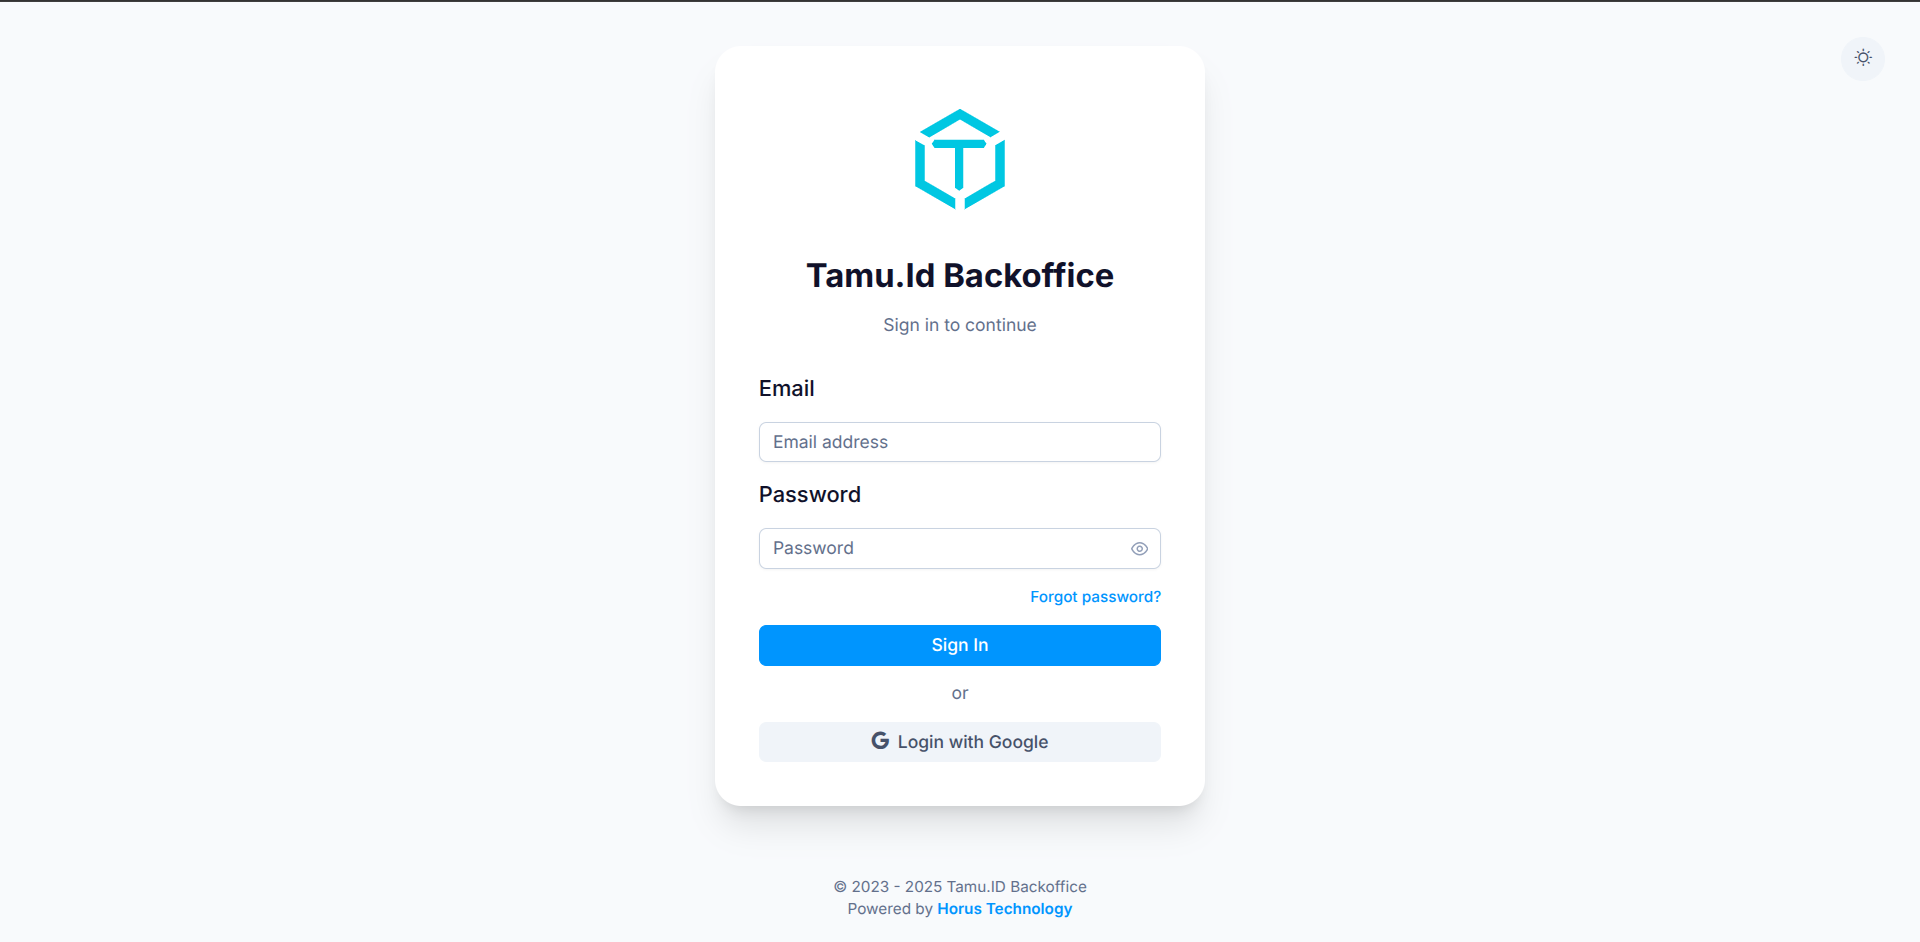
\includegraphics[width=\textwidth]{images/halaman-sa/login.png}
    \caption{Tampilan Halaman Login Admin}
    \label{fig:halaman-login-admin}
\end{figure}

\begin{figure}[H]
    \centering
    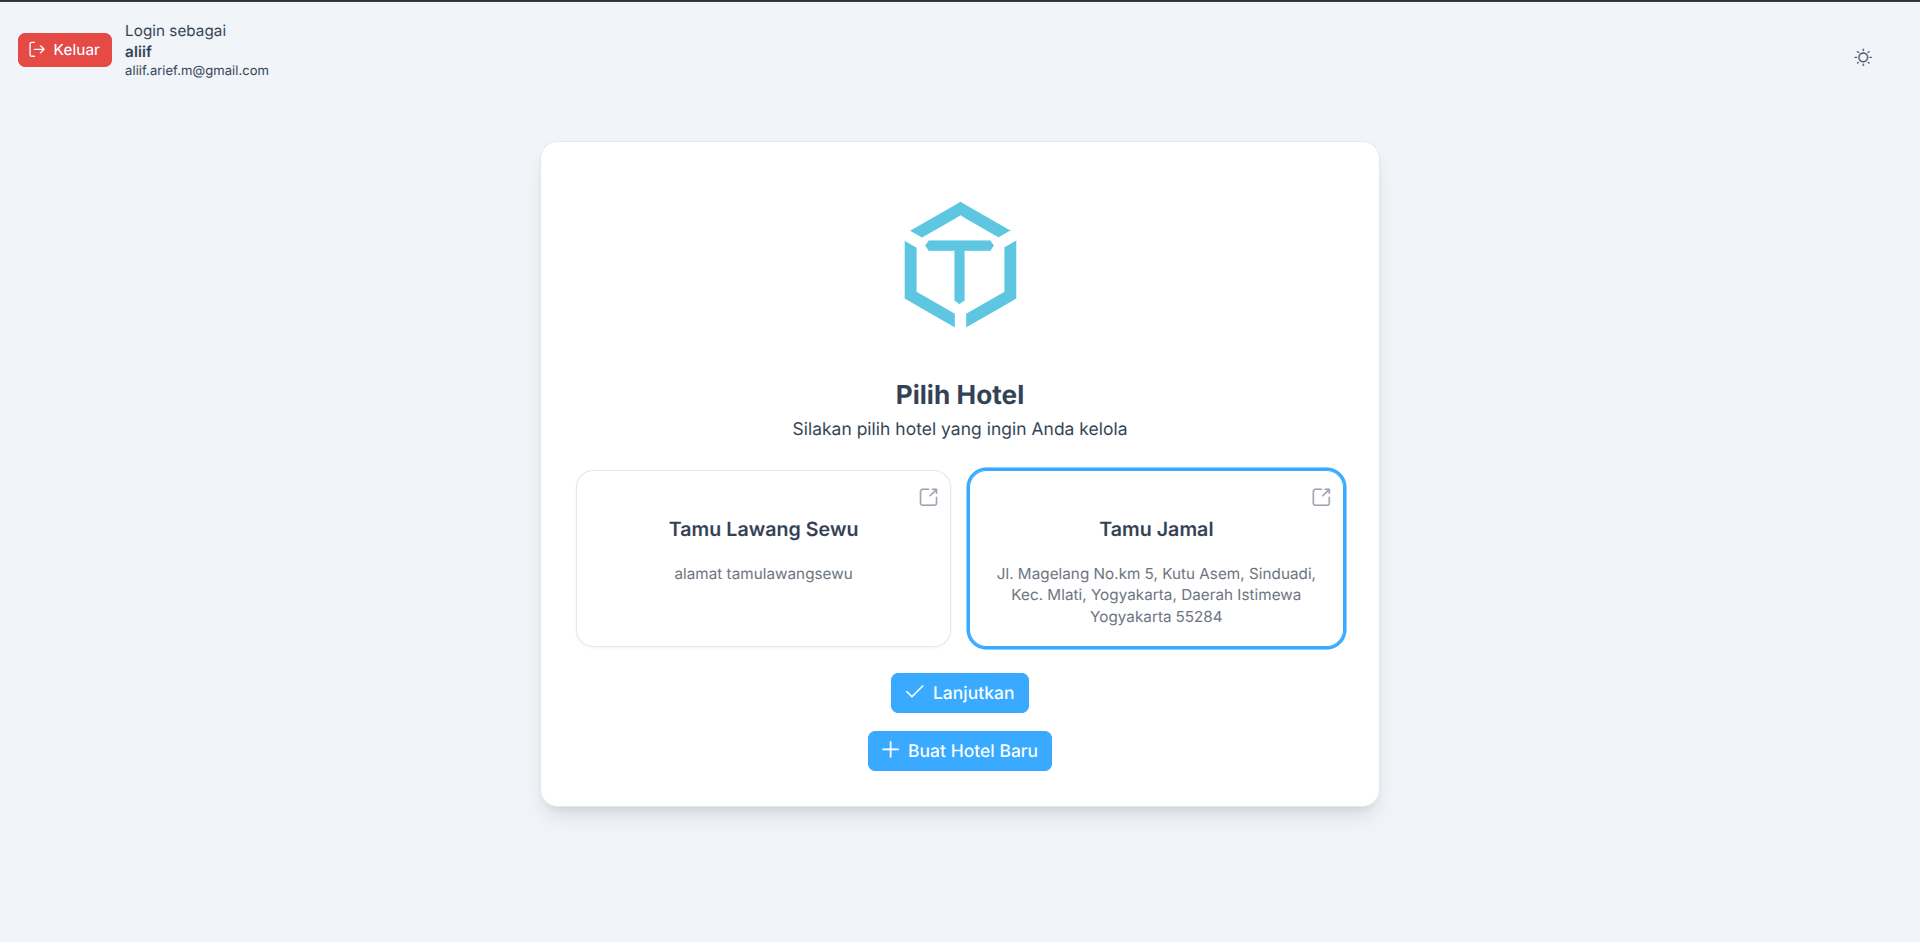
\includegraphics[width=\textwidth]{images/halaman-admin/pilih-cabang.png}
    \caption{Tampilan Halaman Pilih Cabang Admin}
    \label{fig:halaman-pilih-cabang-admin}
\end{figure}

Setelah Admin berhasil login, admin akan diarahkan ke halaman pilih cabang. Pada halaman ini, admin dapat memilih cabang yang akan dikelola. Admin dapat mengelola lebih dari satu cabang, Tampilan halaman pilih cabang admin dapat dilihat pada Gambar \ref{fig:halaman-pilih-cabang-admin}.

\begin{figure}[H]
    \centering
    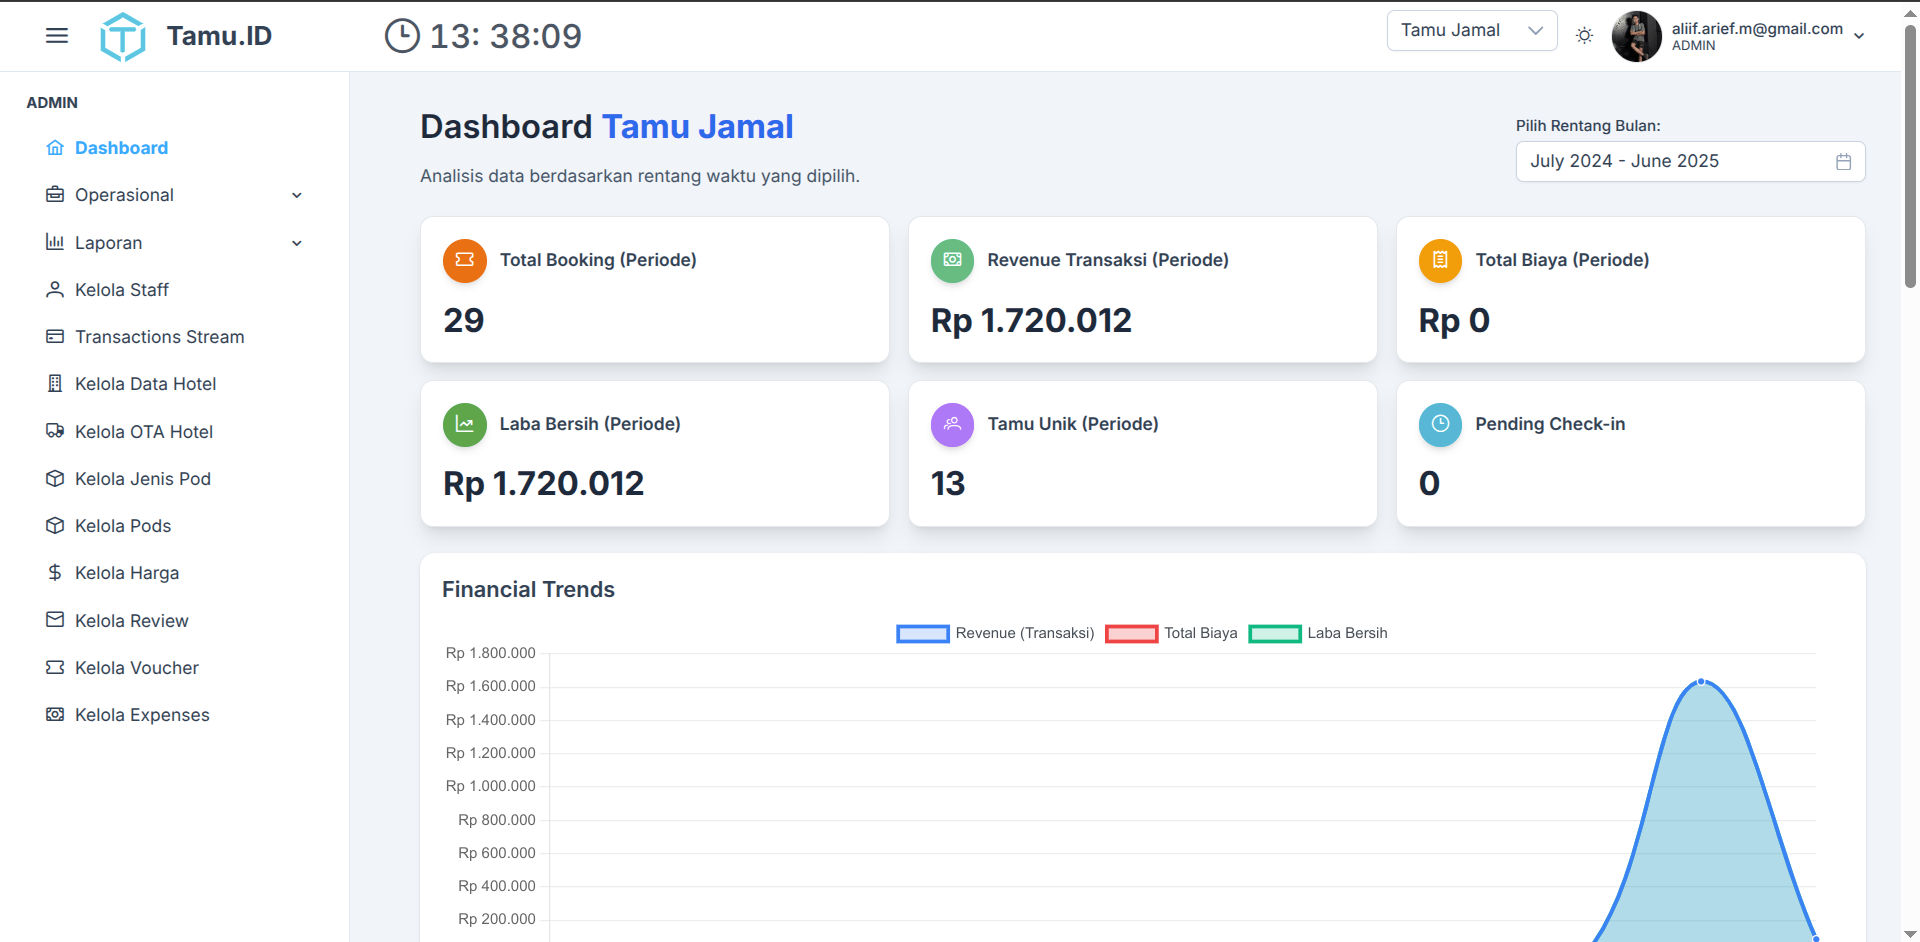
\includegraphics[width=\textwidth]{images/halaman-admin/dasbor.png}
    \caption{Tampilan Halaman Dasbor Admin Cabang}
    \label{fig:halaman-dasbor-admin}
\end{figure}

Setelah memilih cabang, admin akan diarahkan ke halaman dasbor admin cabang. Pada halaman ini, admin dapat melihat informasi garis besar mengenai cabang yang dikelola seperti pada Gambar \ref{fig:halaman-dasbor-admin}.


\begin{figure}[H]
    \centering
    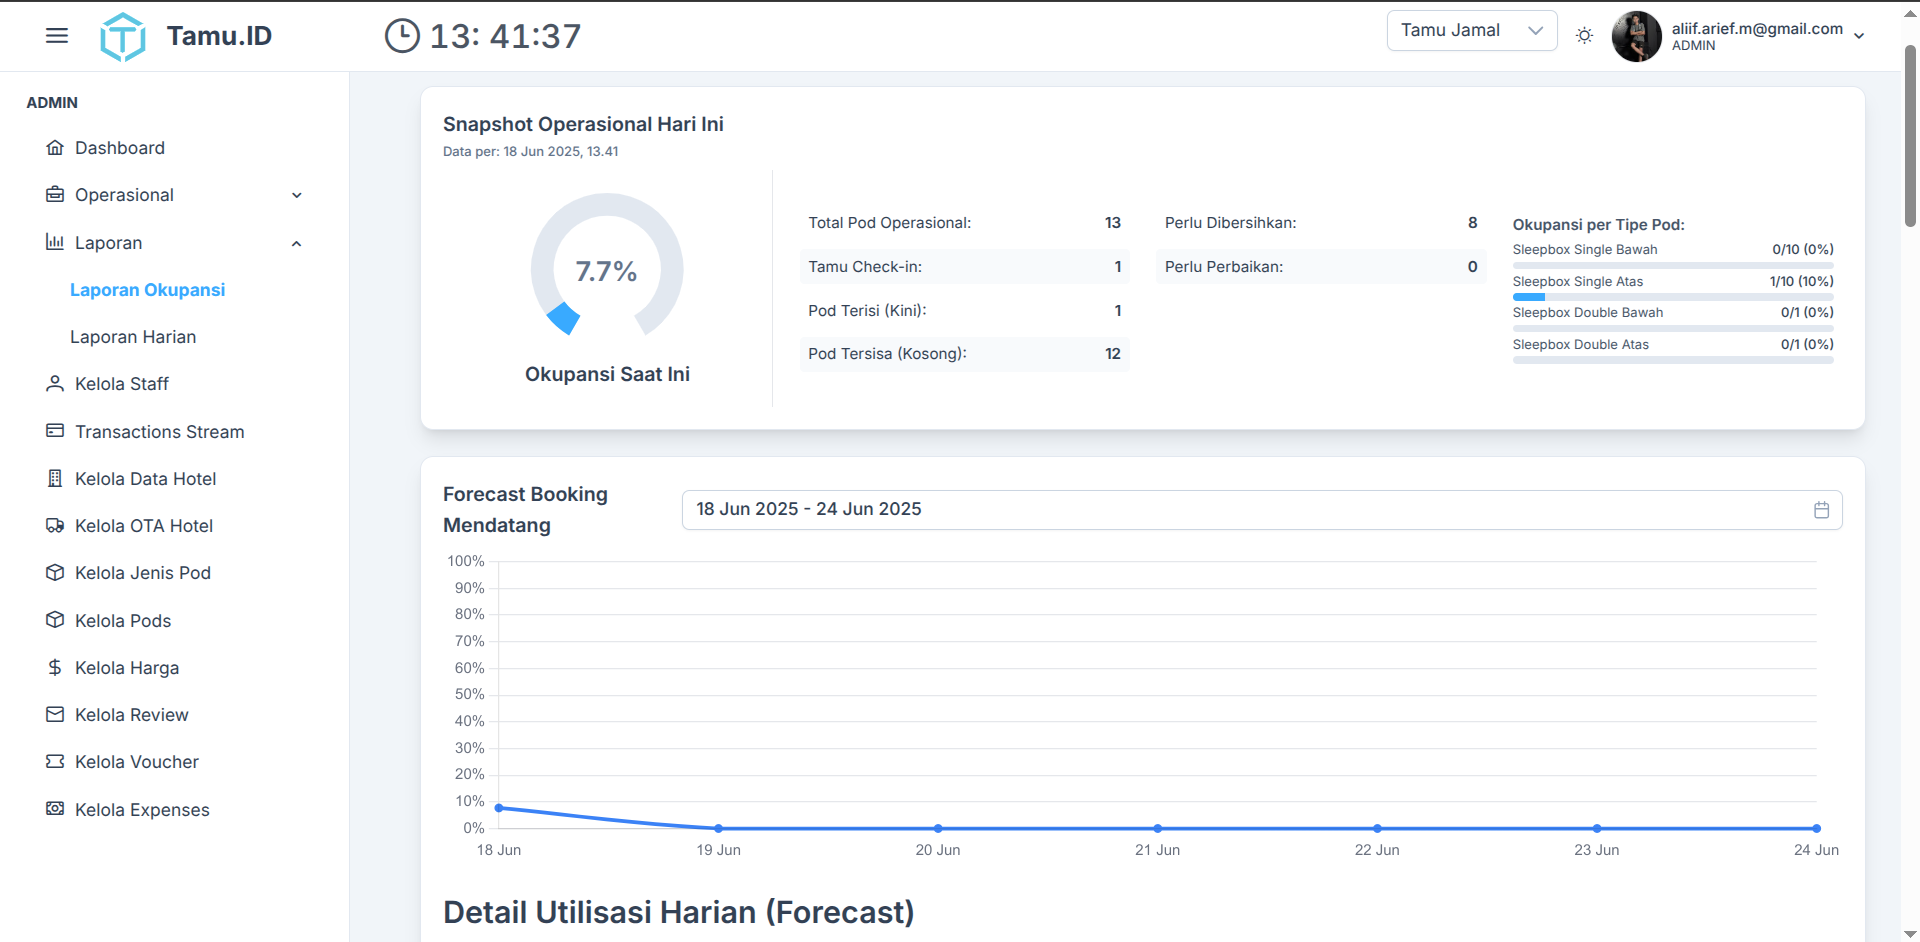
\includegraphics[width=\textwidth]{images/halaman-admin/dasbor-okupansi.png}
    \caption{Tampilan Halaman Dasbor Okupansi Admin Cabang}
    \label{fig:halaman-dasbor-okupansi-admin}
\end{figure}

Pada gambar \ref{fig:halaman-dasbor-okupansi-admin} adalah tampilan halaman dasbor okupansi admin cabang. Pada halaman ini, admin dapat melihat informasi okupansi cabang yang dikelola secara real-time, selain itu juga pada halaman ini admin dapat melihat perkiraan tingkat okupansi beberapa hari ke depan dan juga melihat performa okupansi cabang dalam beberapa hari terakhir. Hal ini dapat membantu admin dalam mengelola okupansi cabang dan membuat keputusan yang lebih baik.


\begin{figure}[H]
    \centering
    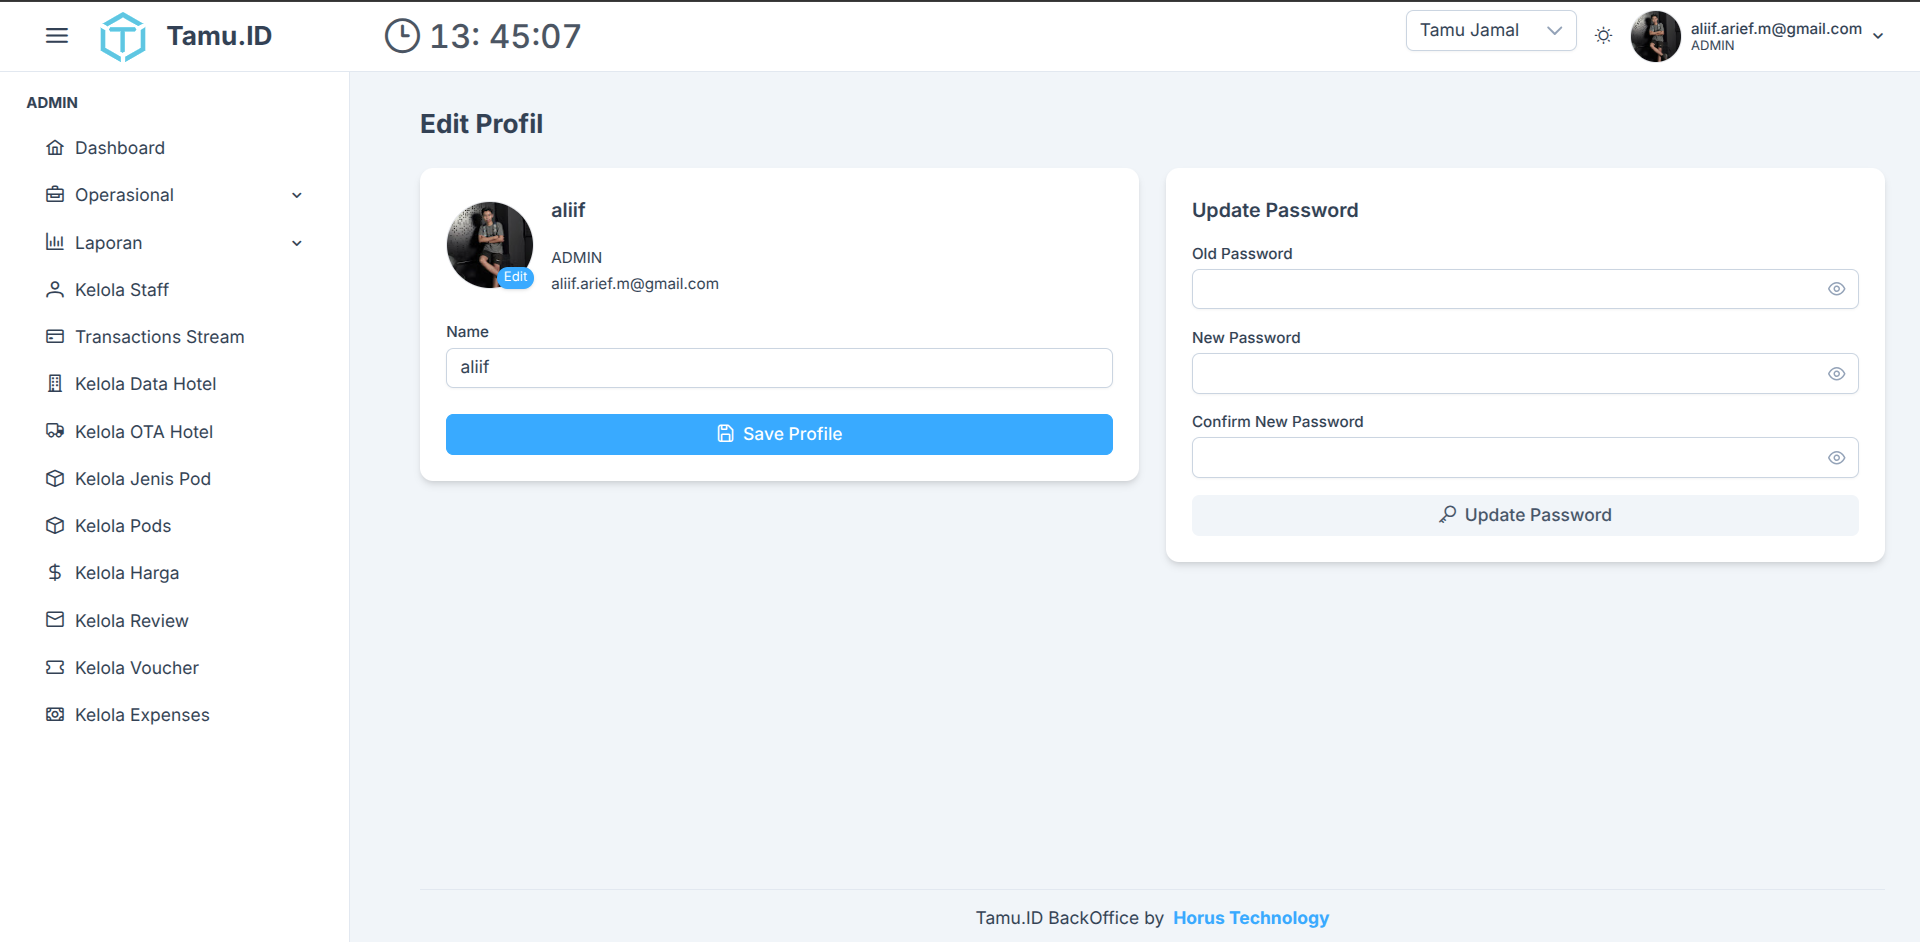
\includegraphics[width=\textwidth]{images/halaman-admin/profil.png}
    \caption{Tampilan Halaman Profil Admin Cabang}
    \label{fig:halaman-profil-admin}
\end{figure}

Pada gambar \ref{fig:halaman-profil-admin} adalah tampilan halaman profil admin cabang. Pada halaman ini, admin dapat melihat informasi profil mereka seperti nama, email, dan nomor telepon. Admin juga dapat mengubah informasi profil mereka jika diperlukan.



\subsubsection{Kelola Data Cabang}

Untuk melakukan update data cabang, admin dapat mengakses halaman kelola data cabang seperti pada gambar \ref{fig:halaman-admin-kelola-cabang} dan \ref{fig:halaman-admin-kelola-cabang-2}.

\begin{figure}[H]
    \centering
    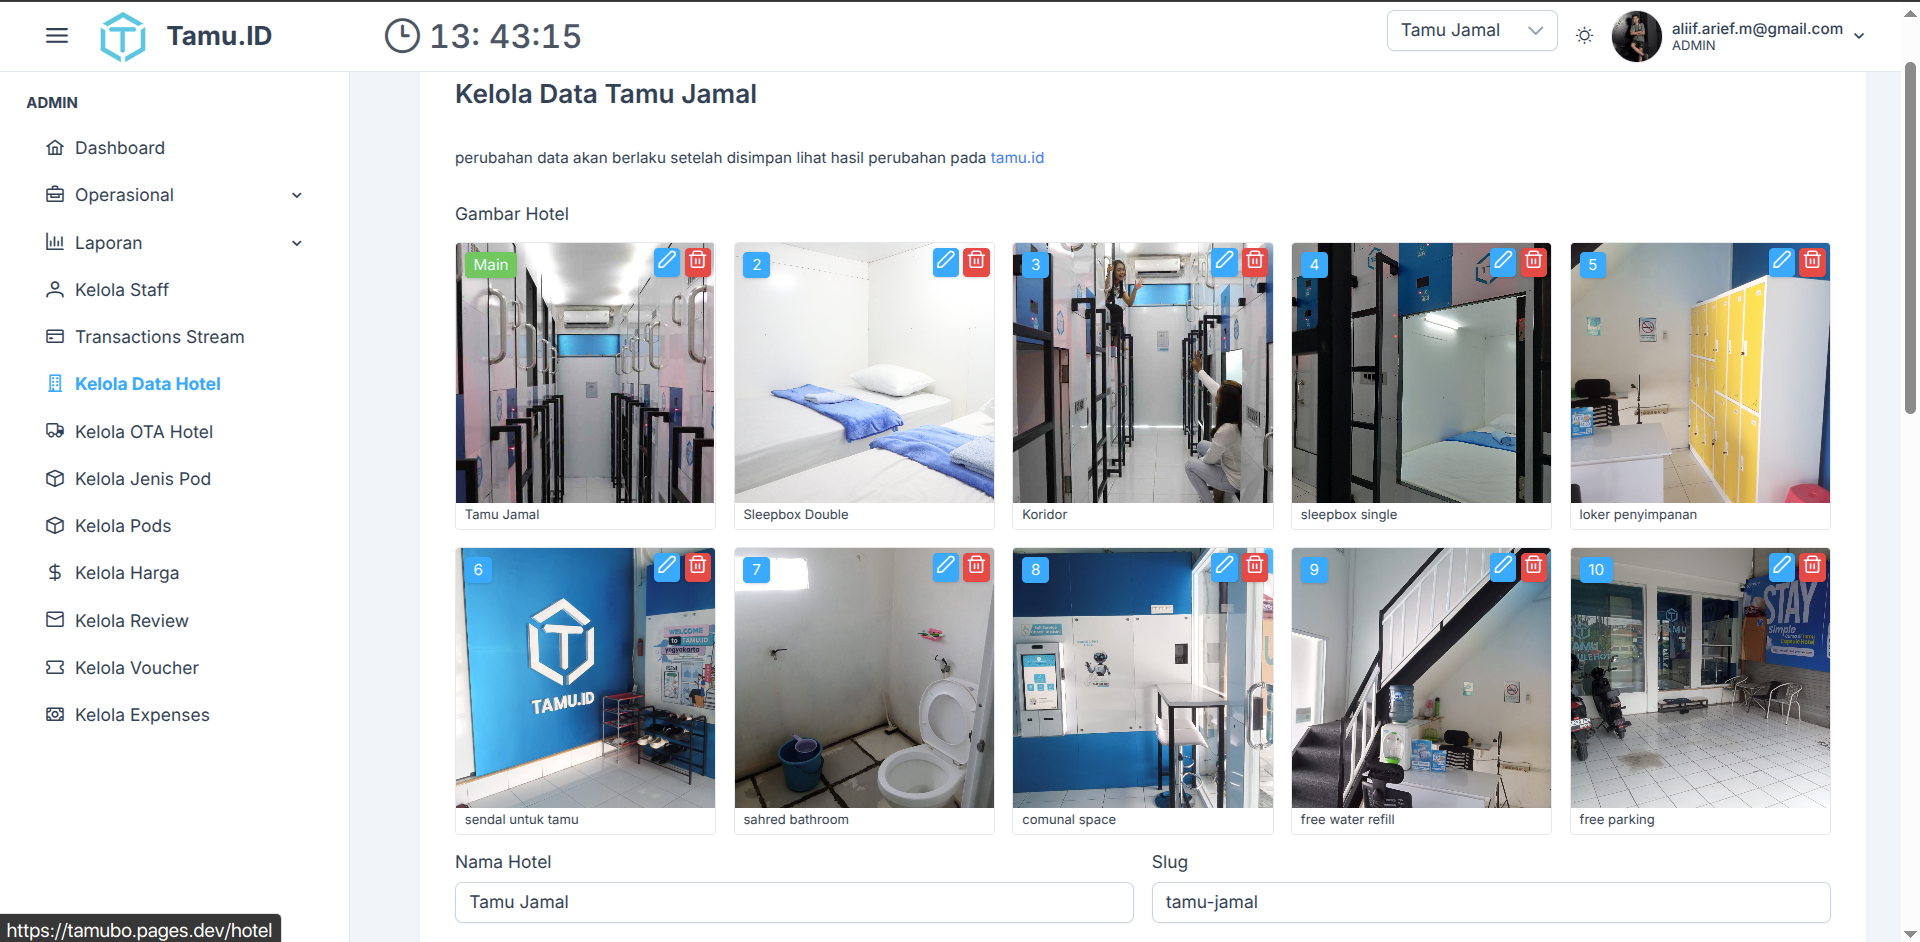
\includegraphics[width=\textwidth]{images/halaman-admin/edit-cabang1.png}
    \caption{Tampilan Admin Kelola Data Cabang}
    \label{fig:halaman-admin-kelola-cabang}
\end{figure}


\begin{figure}[H]
    \centering
    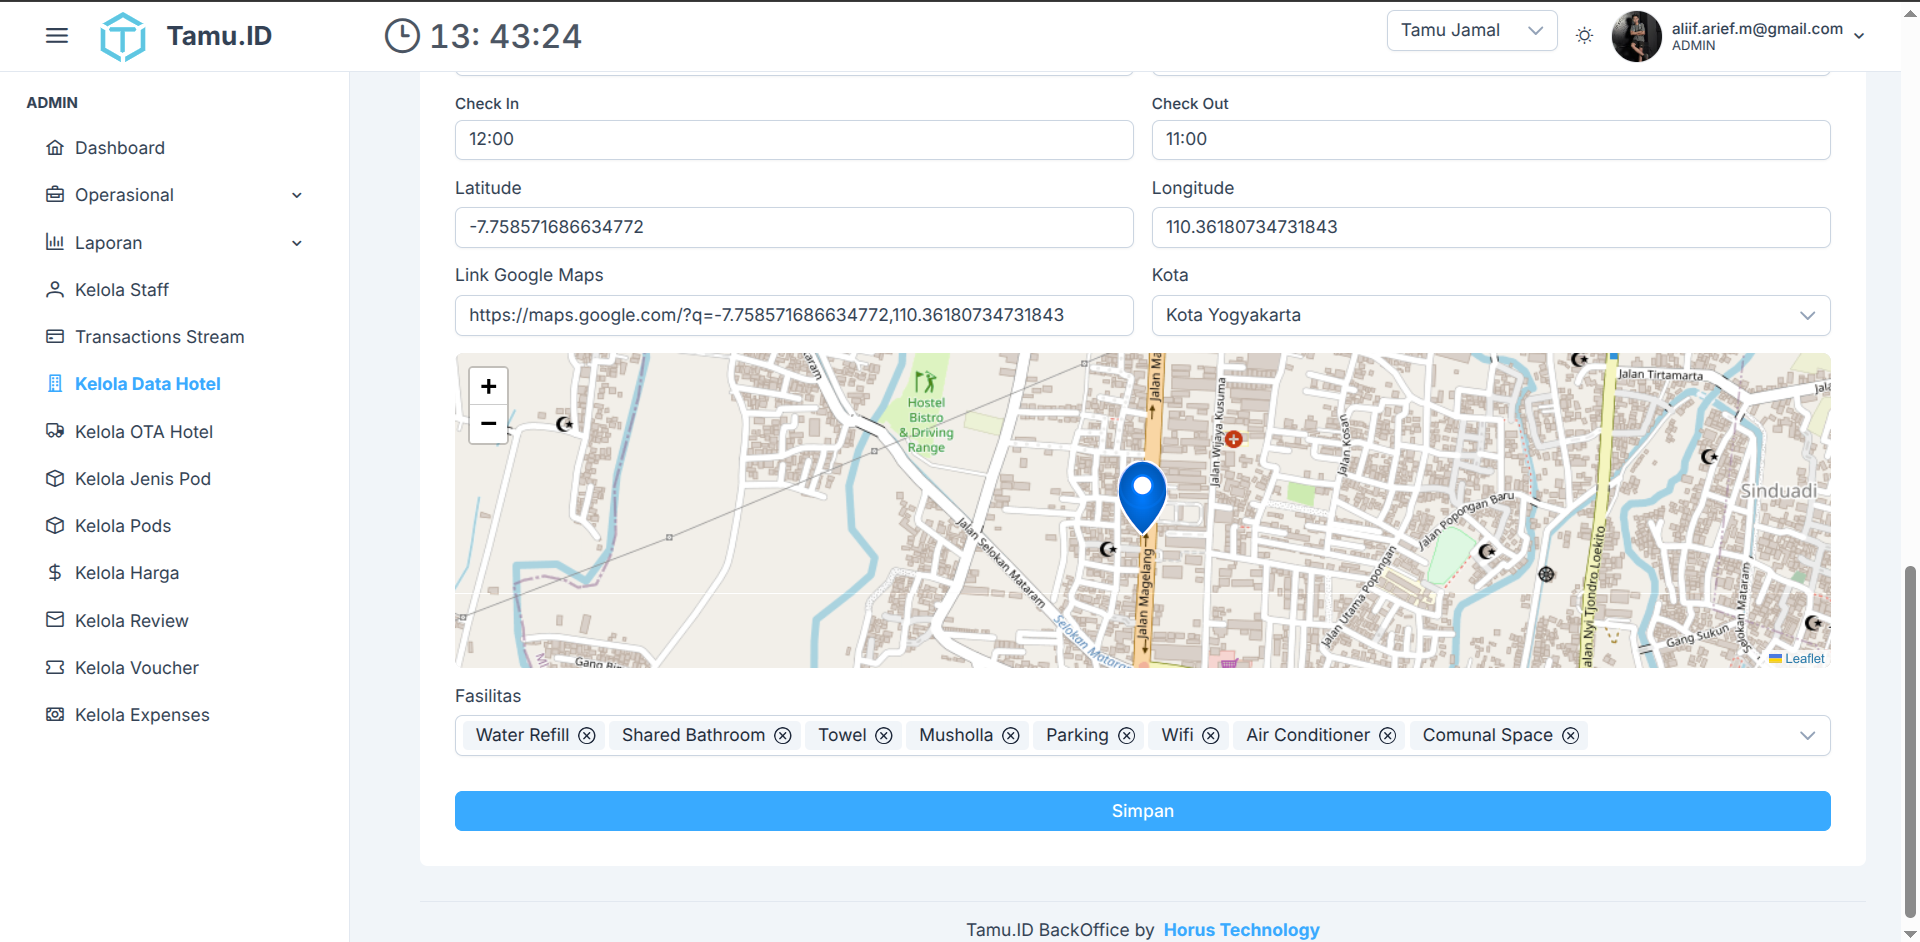
\includegraphics[width=\textwidth]{images/halaman-admin/edit-cabang2.png}
    \caption{Tampilan Admin Kelola Data Cabang}
    \label{fig:halaman-admin-kelola-cabang-2}
\end{figure}

Yang paling utama dari sebuah cabang adalah tiap cabang memiliki jenis pod yang dapat dipesan oleh \textit{User}, oleh karena itu pada gambar \ref{fig:halaman-admin-kelola-jenis-pod} \textit{Admin} dapat mengelola jenis pod yang ada pada cabang yang ia kelola.

\begin{figure}[H]
    \centering
    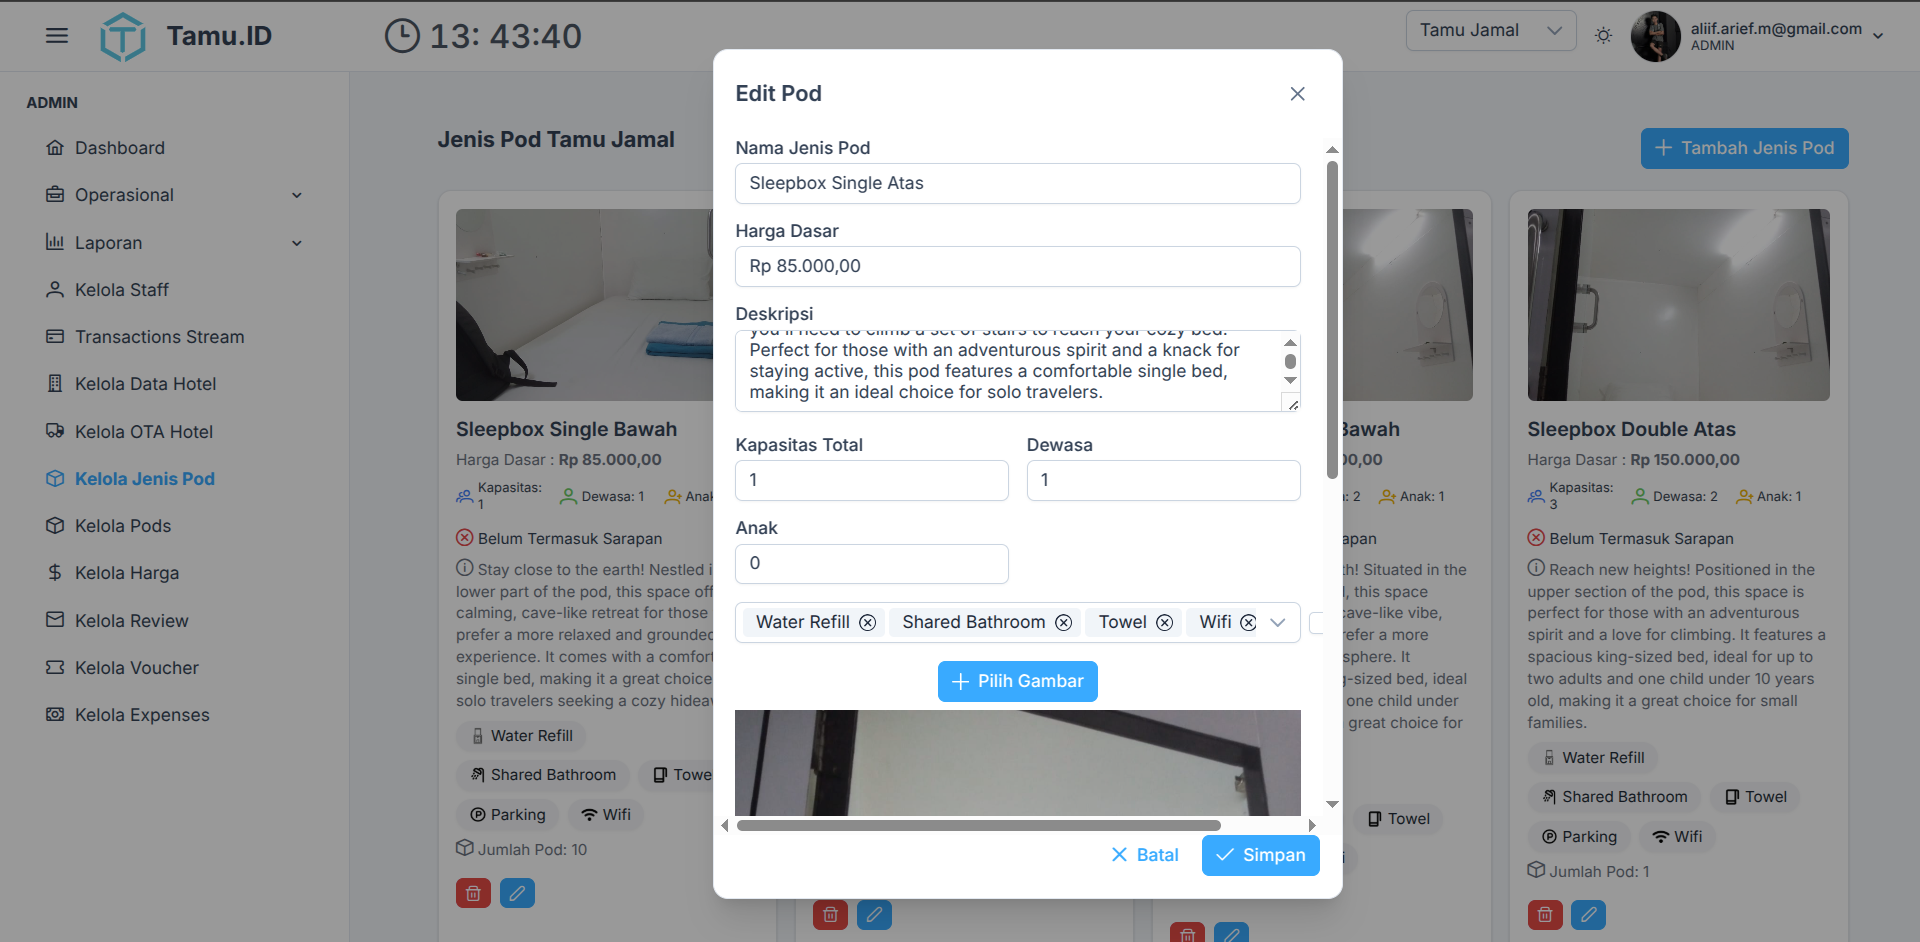
\includegraphics[width=\textwidth]{images/halaman-admin/jenis-pod.png}
    \caption{Tampilan Admin Kelola jenis pod cabang}
    \label{fig:halaman-admin-kelola-jenis-pod}
\end{figure}


Setelah memiliki jenis pod maka selanjutnya untuk masing - masing jenis pod tentunya memiliki anggota yaitu entitas Pod, oleh karena itu \textit{Admin} dapat mengelola Pod yang ada pada cabangnya dari mulai membuat, mengedit, dan menghapusnya sesuai pada gambar \ref{fig:halaman-admin-kelola-pod}.

\begin{figure}[H]
    \centering
    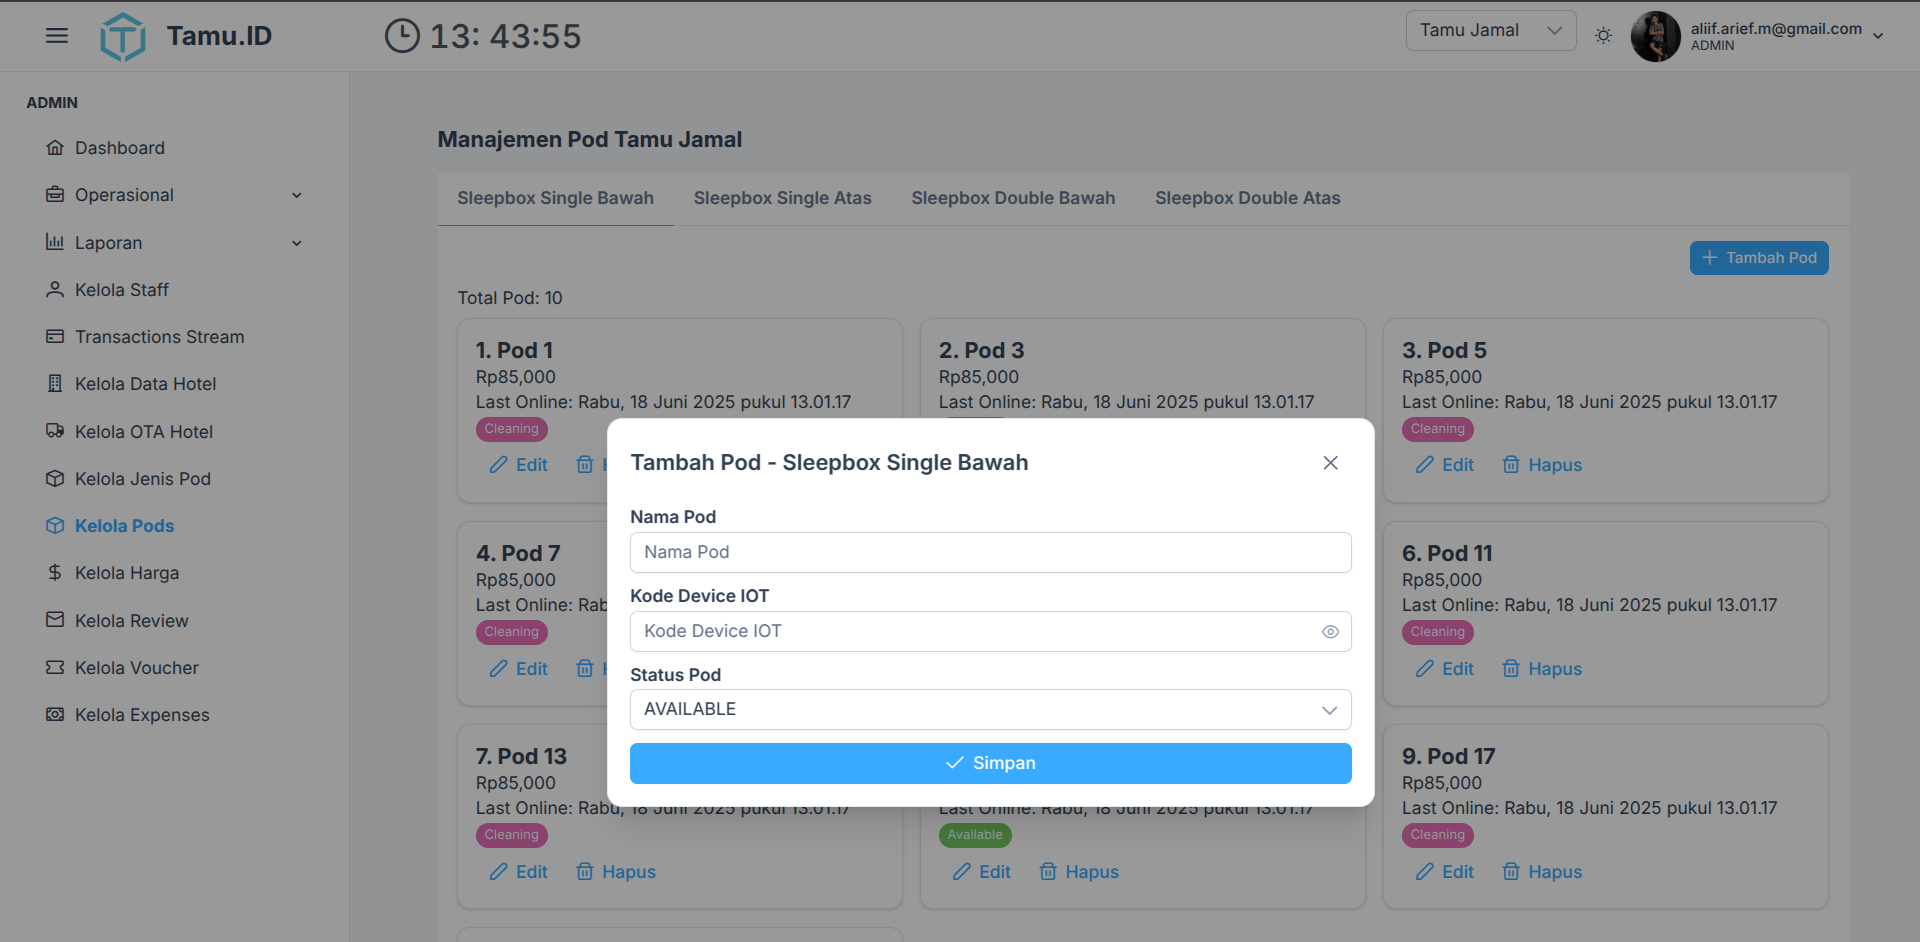
\includegraphics[width=\textwidth]{images/halaman-admin/pod.png}
    \caption{Tampilan Admin Kelola jenis pod cabang}
    \label{fig:halaman-admin-kelola-pod}
\end{figure}

Untuk tiap cabang memiliki kebebasan untuk melakukan integrasi dengan \textit{Online Travel Agency} lain misal Traveloka, Tiket.com, Booking.com, dll. ataupun tidak sama sekali oleh karena itu pada gambar \ref{fig:halaman-admin-kelola-ota} \textit{Admin} dapat mengelola \textit{Online Travel Agency} mana yang aktif pada cabang yang ia kelola.

\begin{figure}[H]
    \centering
    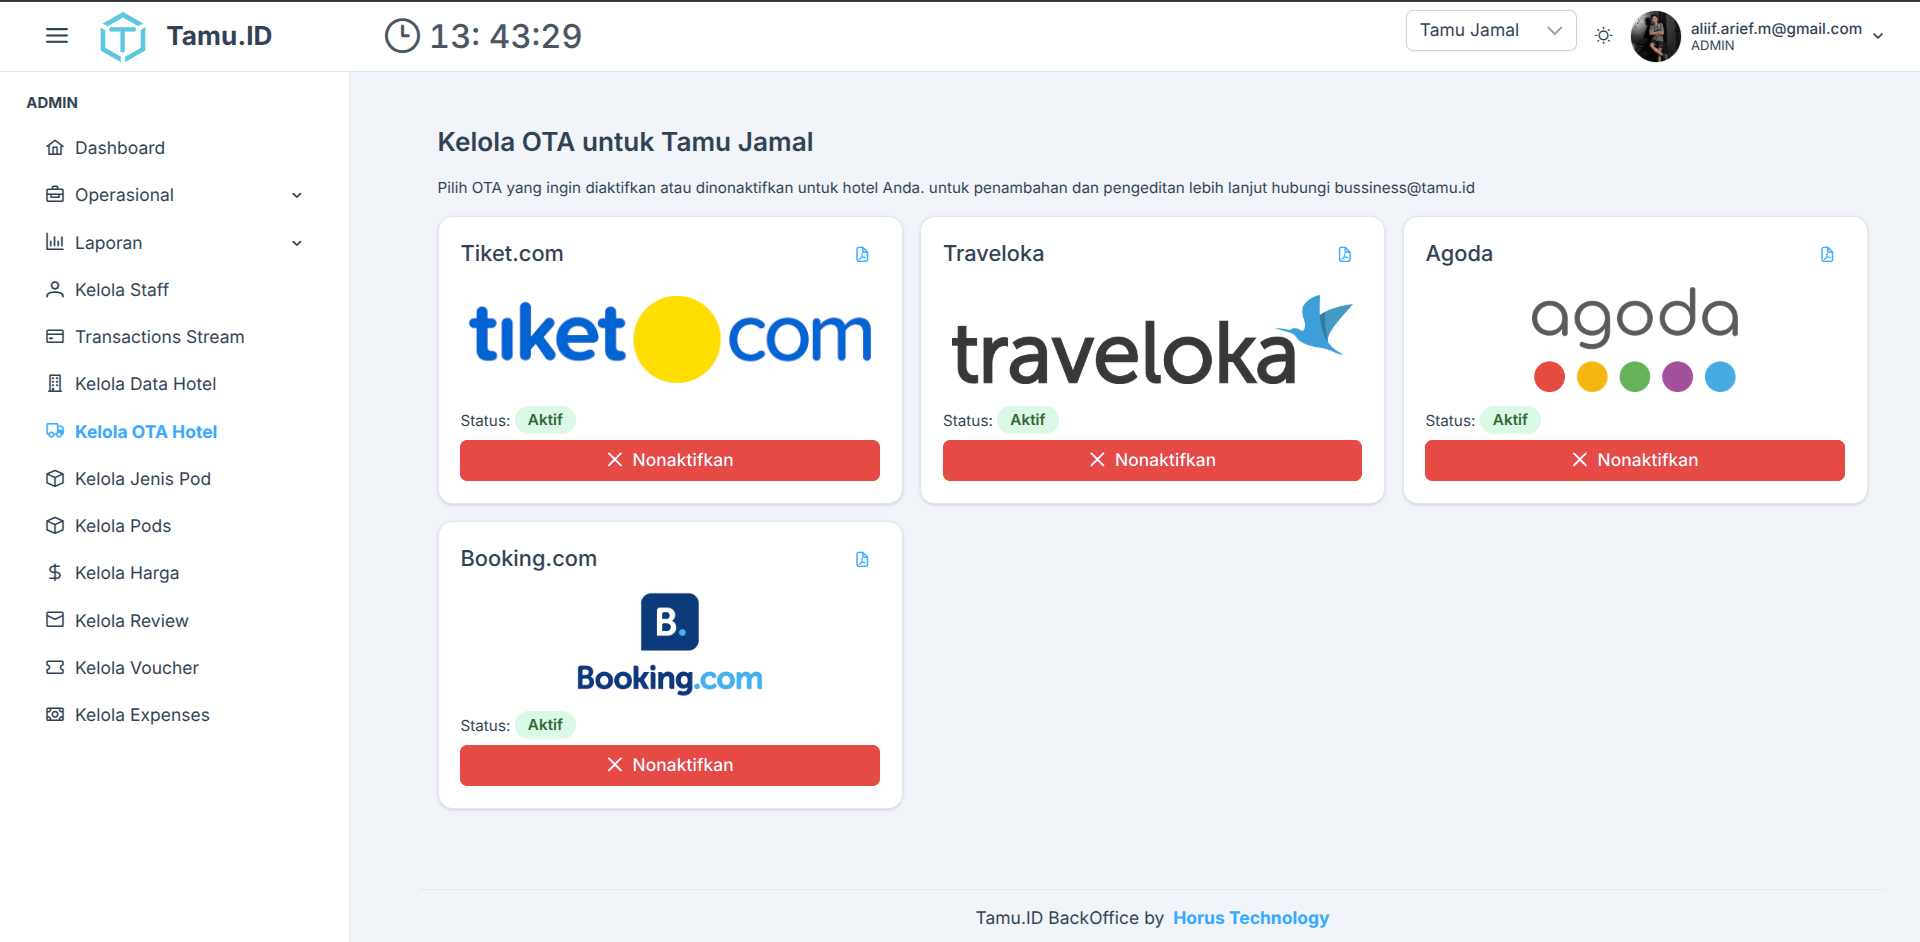
\includegraphics[width=\textwidth]{images/halaman-admin/kelola-ota.png}
    \caption{Tampilan Admin Kelola \textit{OTA} Cabang}
    \label{fig:halaman-admin-kelola-ota}
\end{figure}

Setiap cabang dapat dikelola oleh lebih dari satu Admin atau Staff oleh karena itu pada gambar \ref{fig:halaman-admin-kelola-staff} Staff dengan peran Admin dapat melakukan pengaturan untuk staff pada cabang yang ia kelola.

\begin{figure}[H]
    \centering
    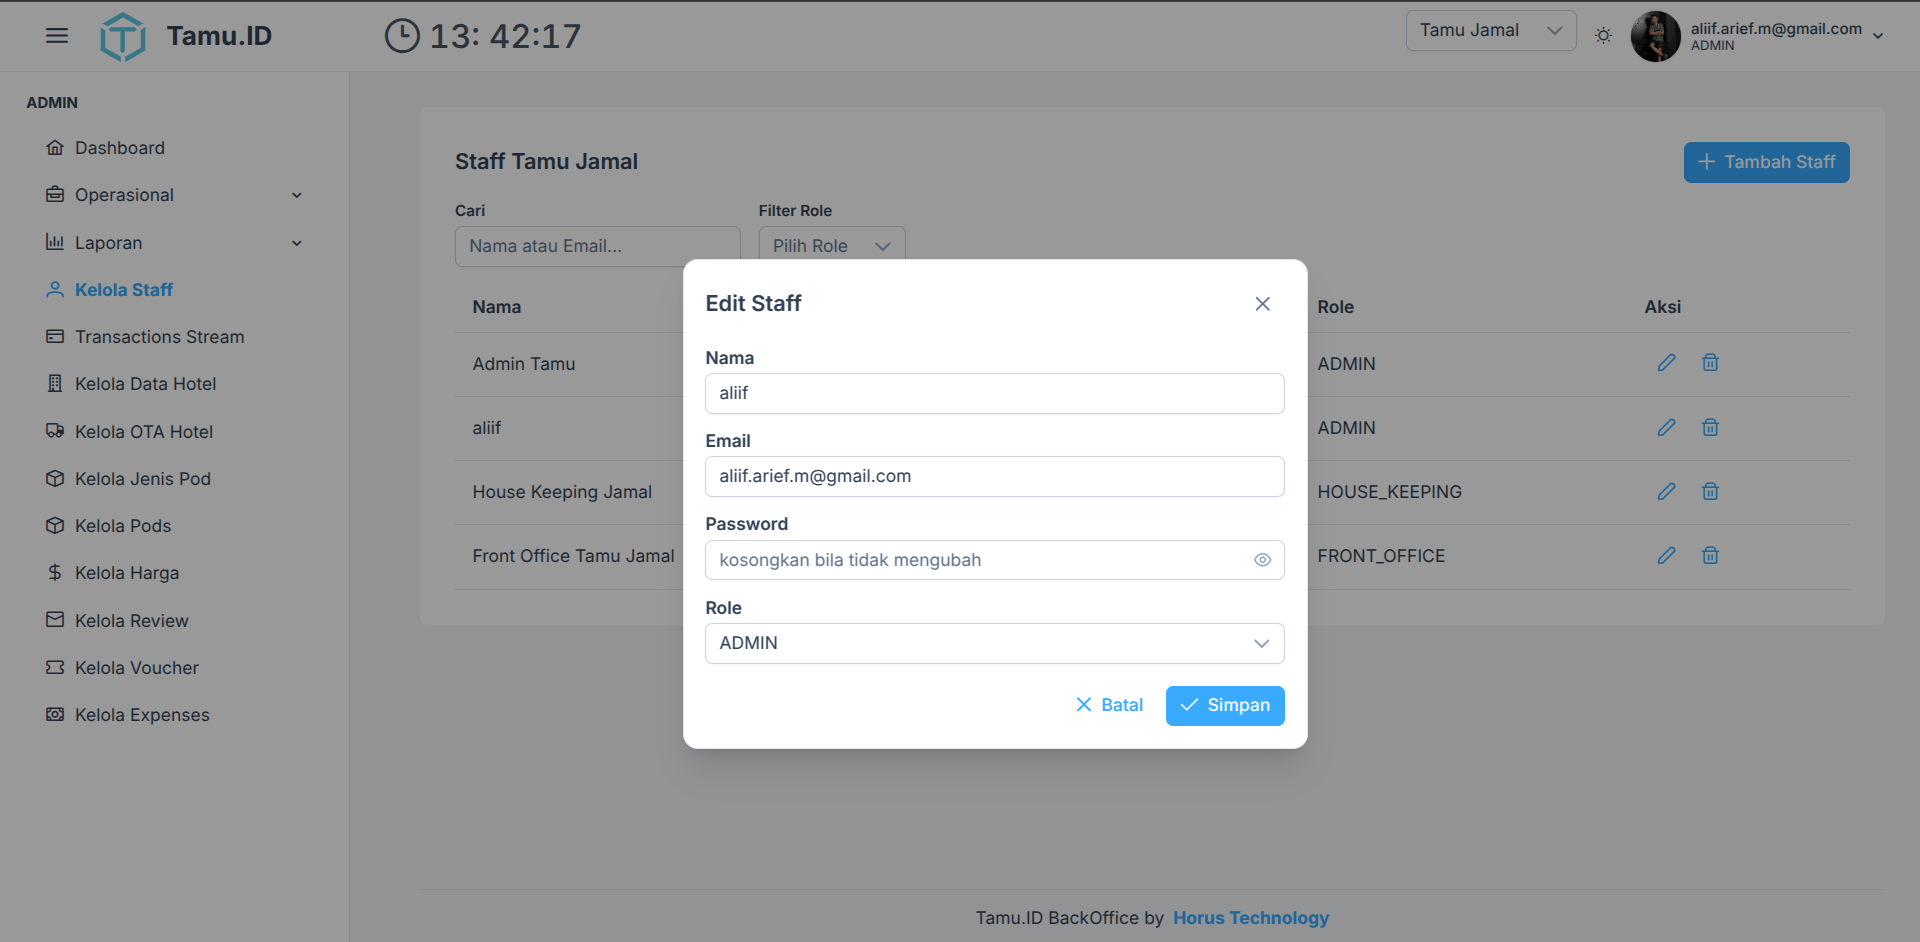
\includegraphics[width=\textwidth]{images/halaman-admin/staff.png}
    \caption{Tampilan Admin Kelola Staff Cabang}
    \label{fig:halaman-admin-kelola-staff}
\end{figure}

Untuk setiap cabang dapat mengadakan promo mandiri yaitu seperti pada gambar \ref{fig:halaman-admin-kelola-voucher}, Admin dapat membuat Voucher promo khusus untuk cabang yang ia kelolal.

\begin{figure}[H]
    \centering
    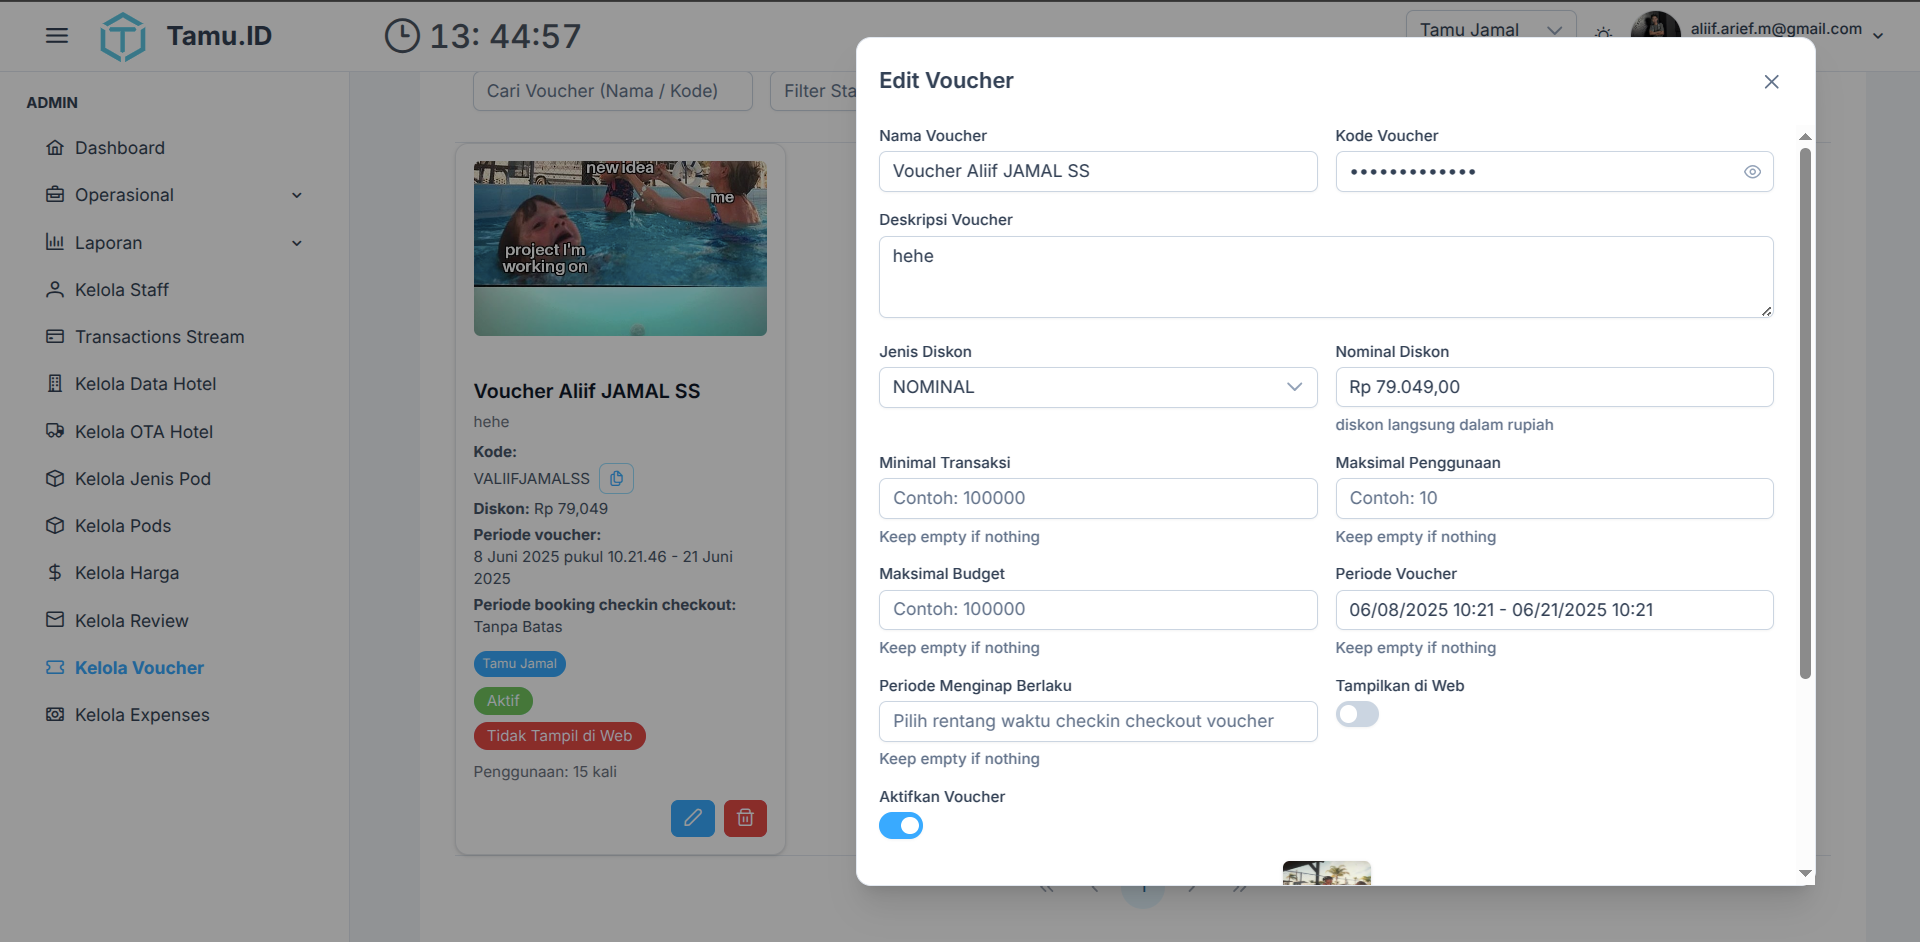
\includegraphics[width=\textwidth]{images/halaman-admin/voucher.png}
    \caption{Tampilan Admin Kelola Voucher Cabang}
    \label{fig:halaman-admin-kelola-voucher}
\end{figure}

Setelah \textit{User} menginap pada suatu Pod maka selanjutnya \textit{User} akan melakukan \textit{Checkout} dan meninggalkan \textit{Review} dan \textit{Review} tentang pengalamannya selama menggunakan layanan, oleh karena itu untuk menghindari \textit{Spam} pada gambar \ref{fig:halaman-admin-kelola-review}, Admind dapat mengelola dan mengontrolnya.

\begin{figure}[H]
    \centering
    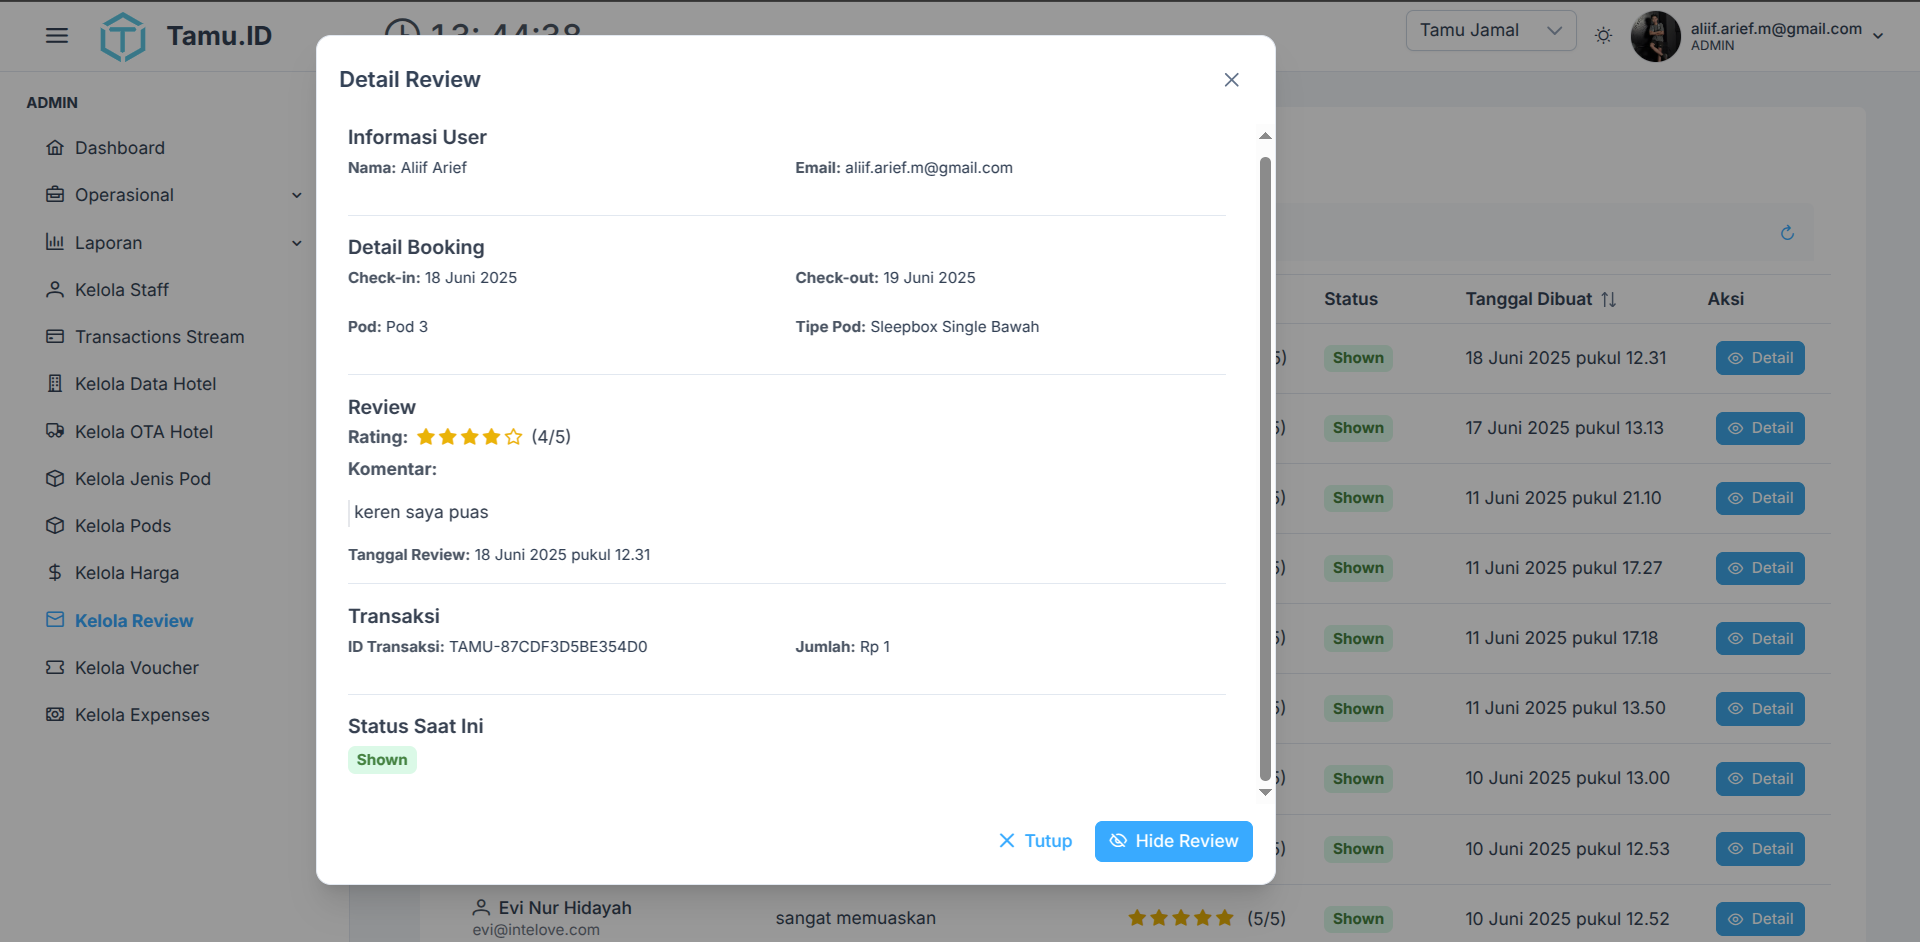
\includegraphics[width=\textwidth]{images/halaman-admin/review.png}
    \caption{Tampilan Admin Kelola Review Cabang}
    \label{fig:halaman-admin-kelola-review}
\end{figure}




\subsubsection{Operasional Harian Cabang}

Untuk mempermudah operasional harian cabang pada gambar \ref{fig:halaman-laporan-harian-admin} admin dapat melihat laporan harian cabang yang dikelola seperti siapa saja yang akan check-in, siapa saja yang sudah check-in, dan siapa saja yang sudah check-out. Hal ini dapat membantu admin dalam mengelola operasional harian cabang dan memastikan bahwa semua diketahui lebih awal oleh admin.

\begin{figure}[H]
    \centering
    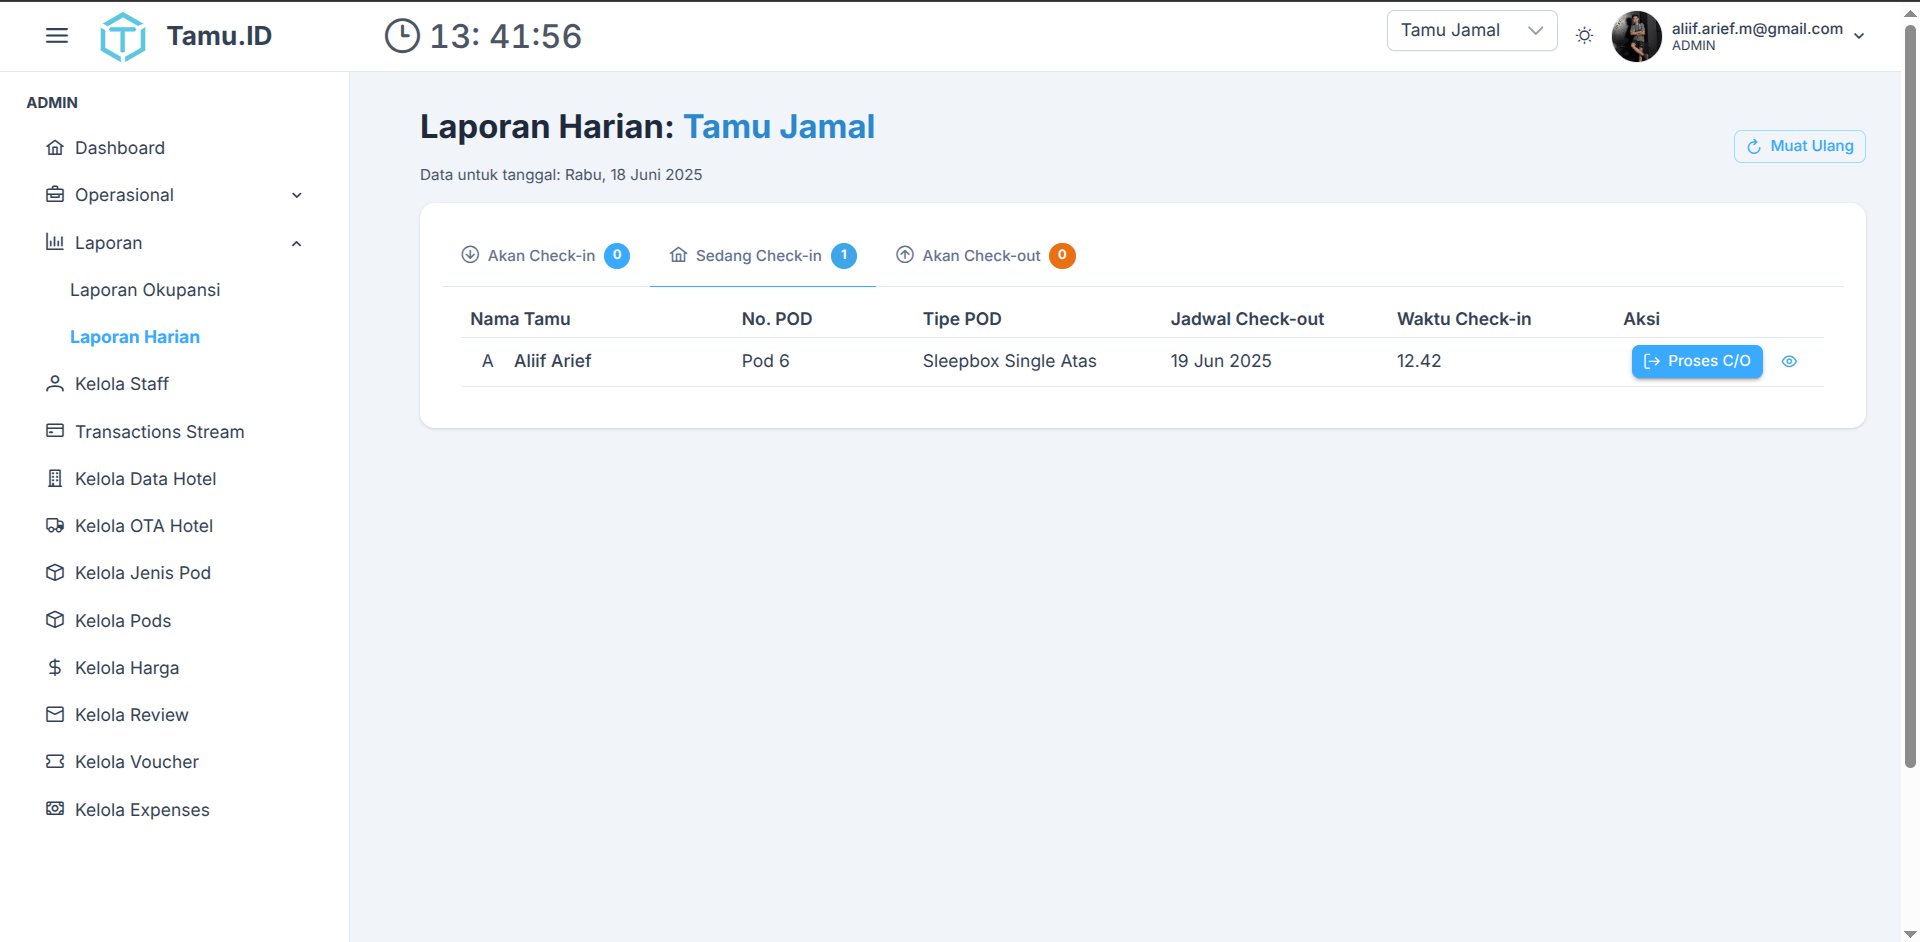
\includegraphics[width=\textwidth]{images/halaman-admin/laporan-harian.png}
    \caption{Tampilan Halaman Laporan Harian Admin Cabang}
    \label{fig:halaman-laporan-harian-admin}
\end{figure}

Pada gambar \ref{fig:halaman-daftar-checkedin-admin} adalah tampilan halaman daftar tamu yang sudah check-in. Pada halaman ini, admin dapat melihat daftar tamu yang sudah check-in pada cabang yang dikelola. Admin juga dapat melakukan tindakan seperti memindahkan tamu ke pod lain jika diperlukan. Hal ini dapat membantu admin dalam mengelola tamu yang sudah check-in dan memastikan bahwa semua tamu terlayani dengan baik.

\begin{figure}[H]
    \centering
    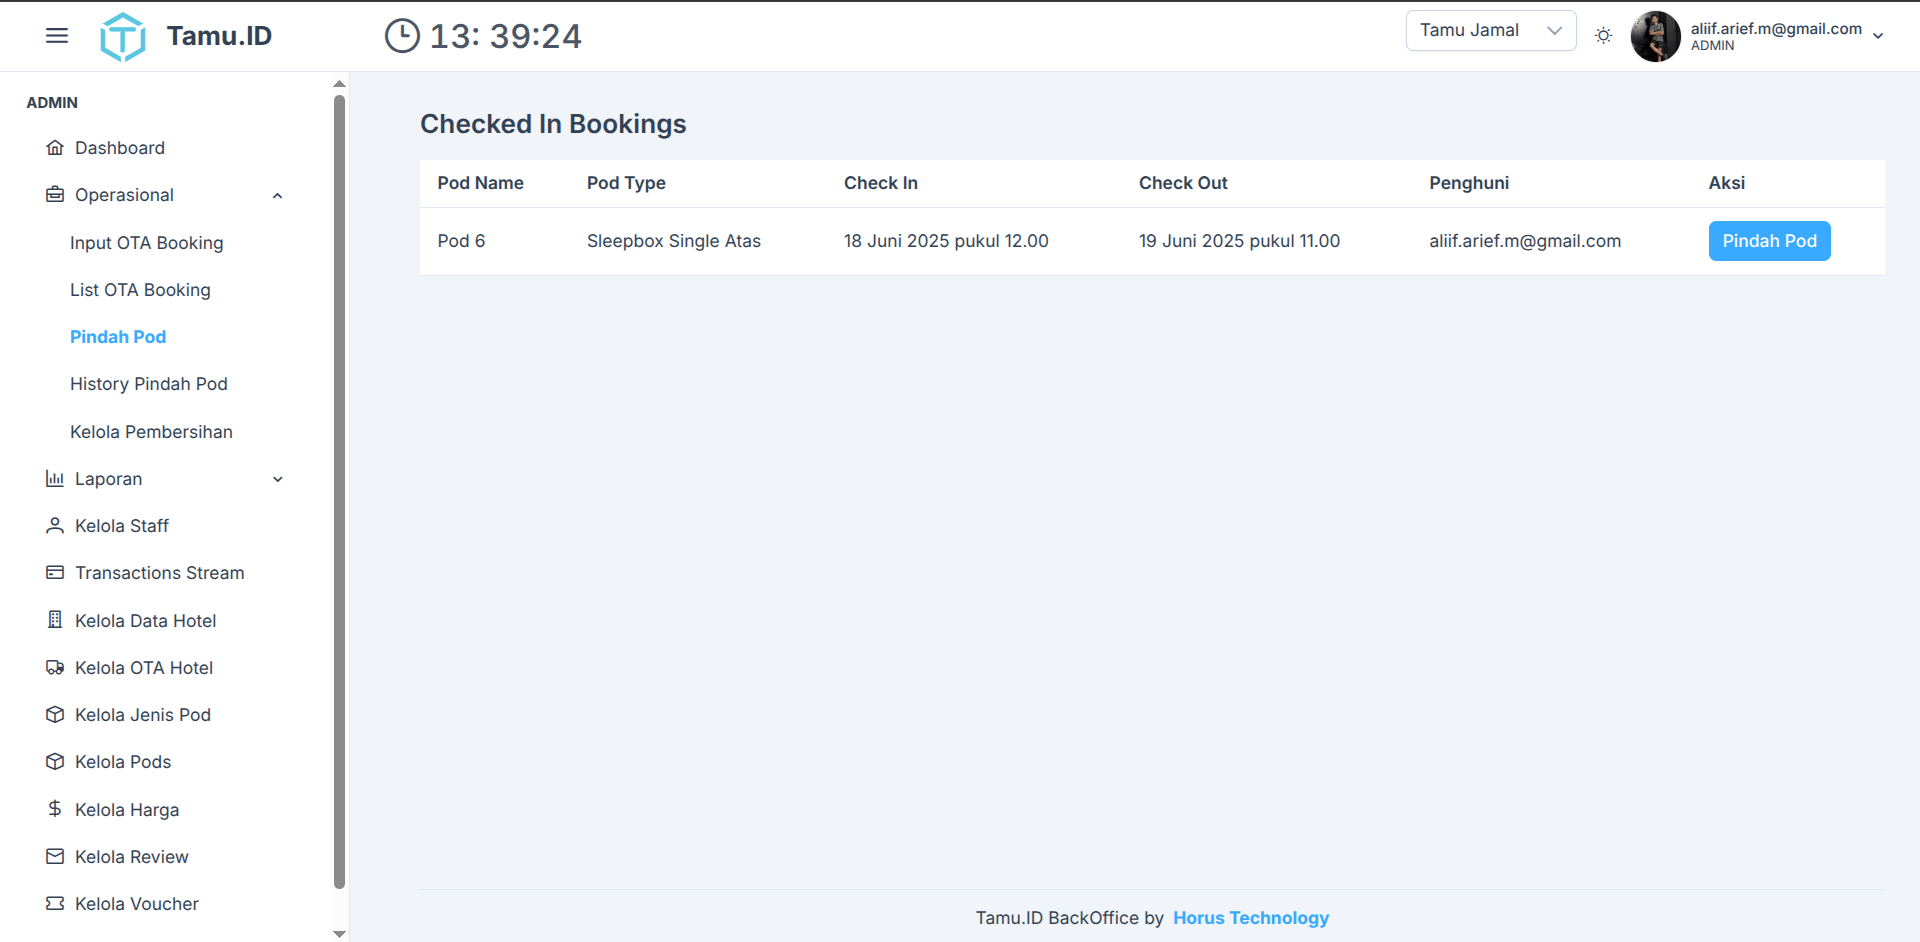
\includegraphics[width=\textwidth]{images/halaman-admin/lis-checkedin.png}
    \caption{Tampilan Halaman Daftar Tamu Check-in Admin Cabang}
    \label{fig:halaman-daftar-checkedin-admin}
\end{figure}

\begin{figure}[H]
    \centering
    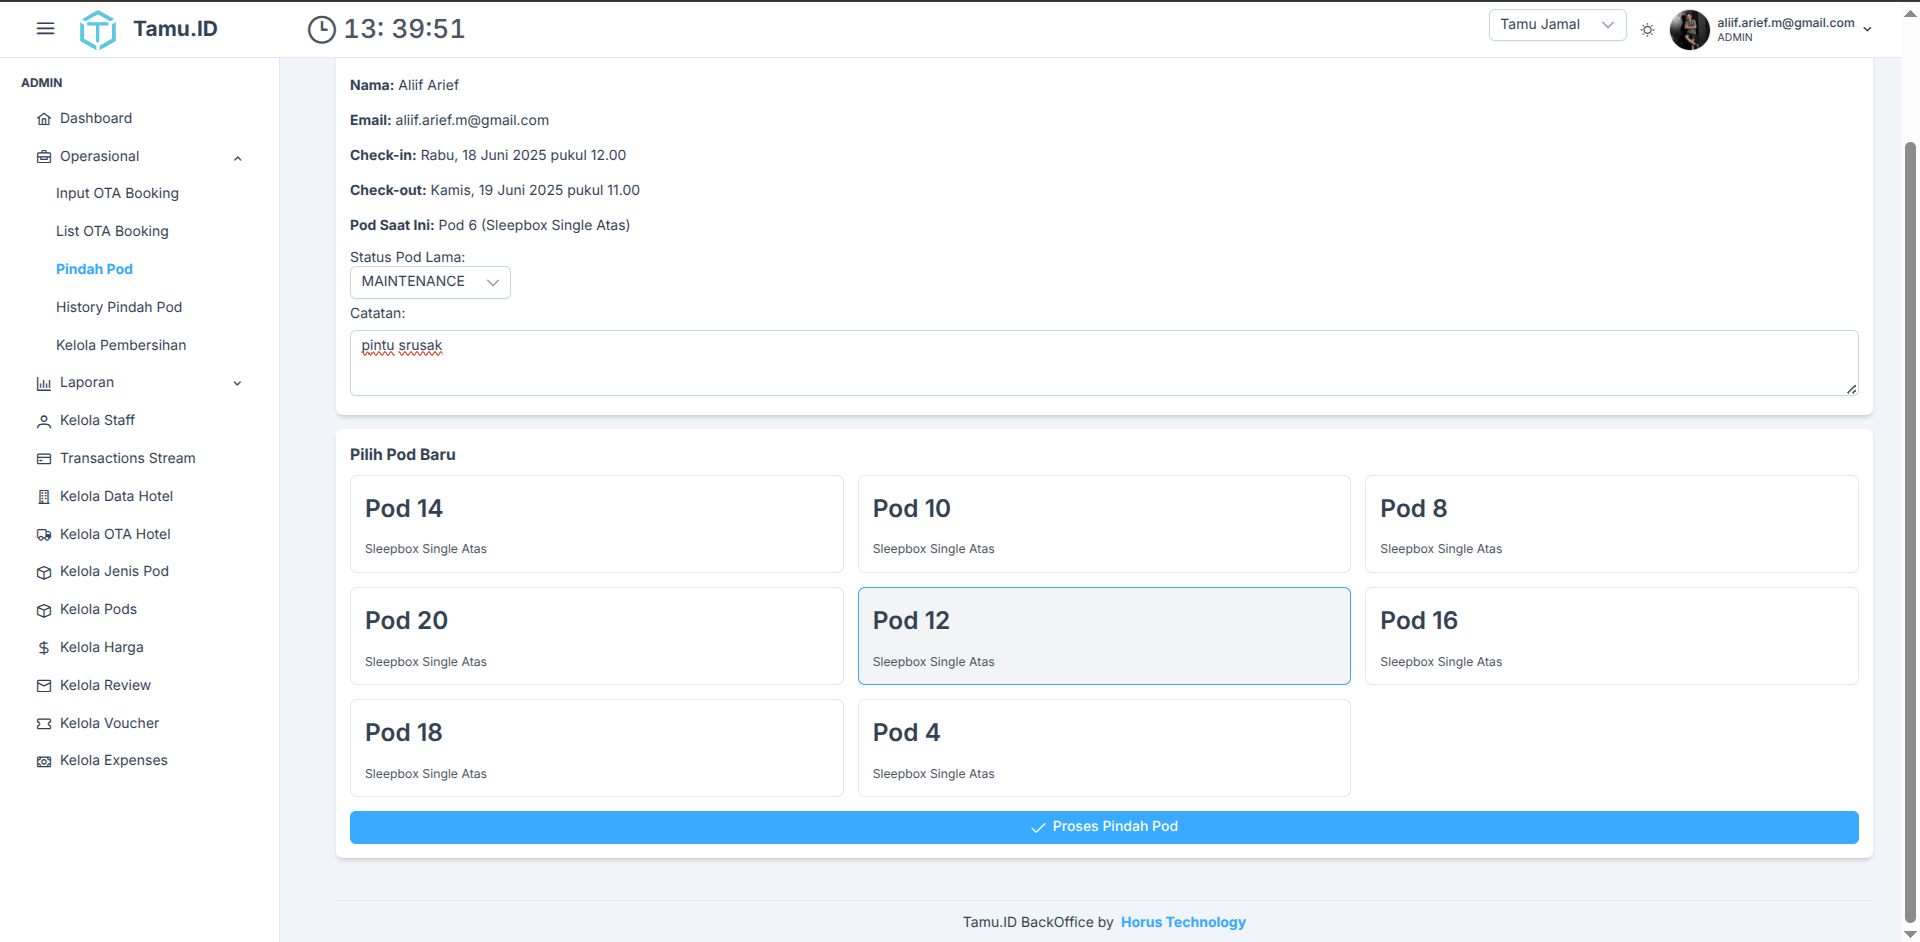
\includegraphics[width=\textwidth]{images/halaman-admin/proses-pindah-pod.png}
    \caption{Tampilan Halaman Proses Pindah Pod User oleh Admin Cabang}
    \label{fig:halaman-proses-pindah-pod-admin}
\end{figure}

Pada gambar \ref{fig:halaman-proses-pindah-pod-admin} adalah tampilan halaman proses pindah pod user oleh admin cabang. Pada halaman ini, admin dapat memindahkan tamu ke pod lain jika diperlukan. status dari pod lama yang ditempati user juga dapat disesuaikan dengan alasan pemindahan tersebut.

\begin{figure}[H]
    \centering
    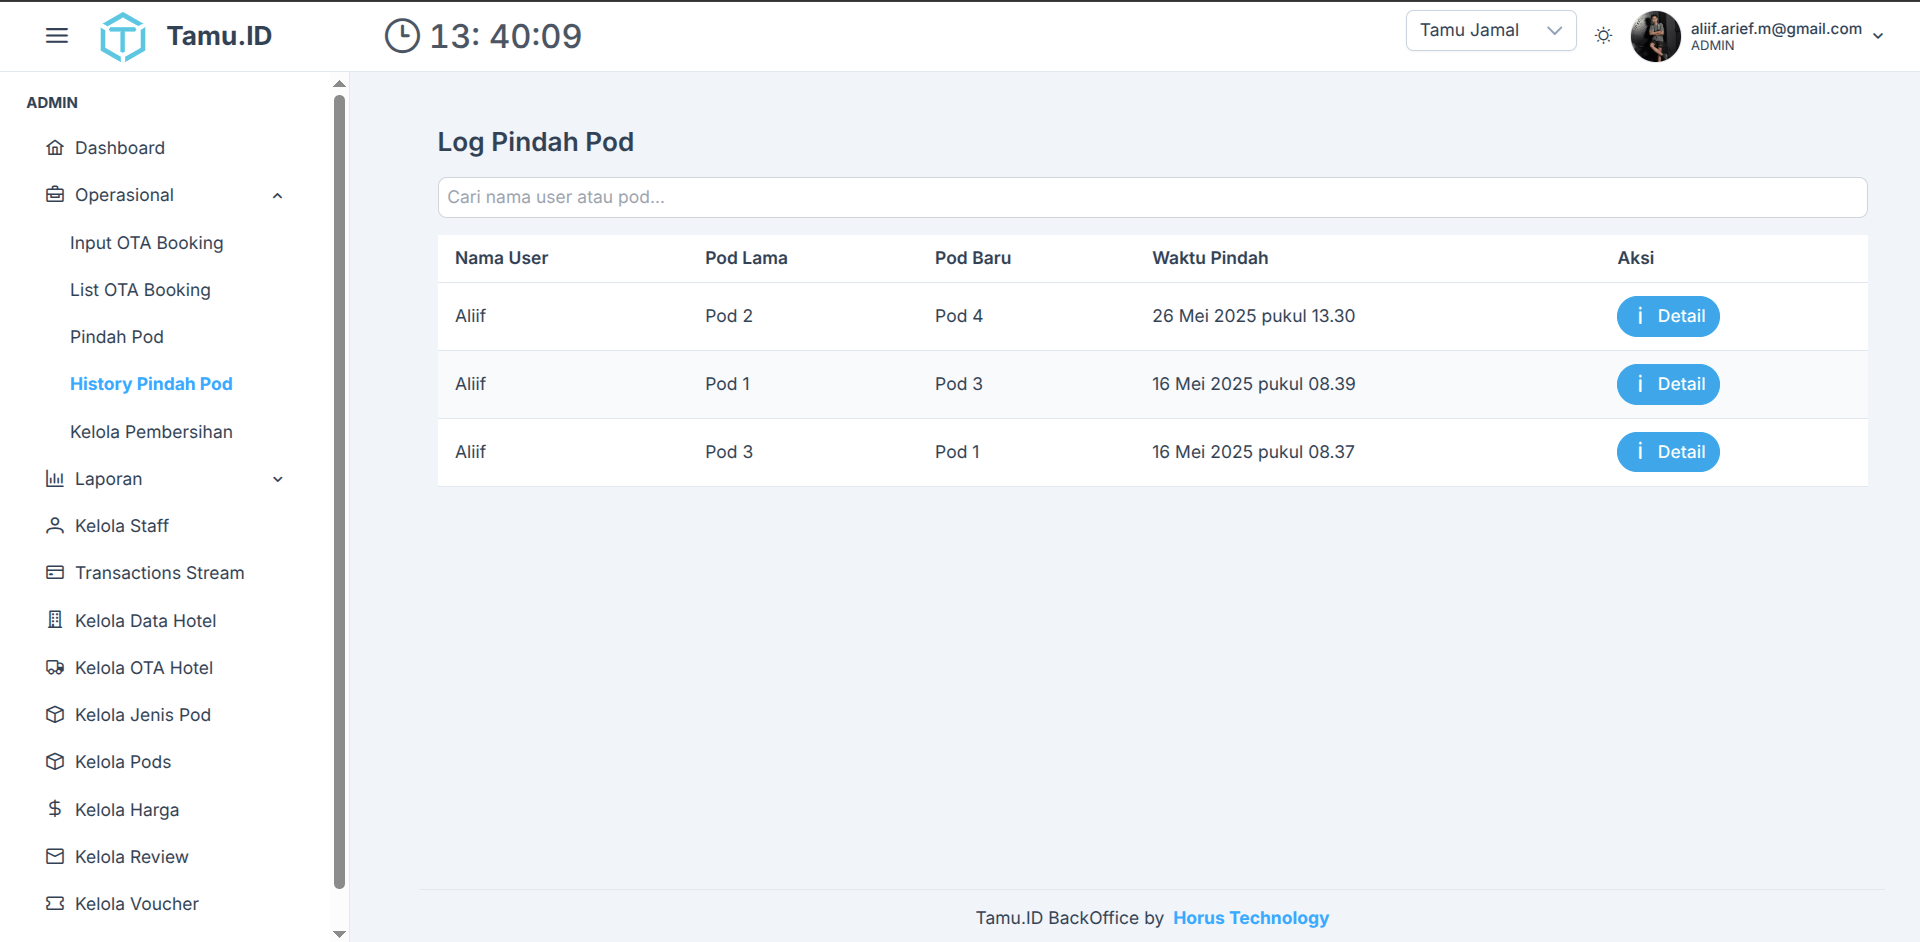
\includegraphics[width=\textwidth]{images/halaman-admin/log-pindah-pod.png}
    \caption{Tampilan Halaman Riwayat Pindah Pod pada Cabang}
    \label{fig:halaman-riwayat-pindah-pod-admin}
\end{figure}

Untuk melihat riwayat pindah pod pada cabang, admin dapat mengakses halaman riwayat pindah pod seperti pada gambar \ref{fig:halaman-riwayat-pindah-pod-admin}. Pada halaman ini, admin dapat melihat riwayat pindah pod yang dilakukan oleh admin pada cabang yang dikelola.


\begin{figure}[H]
    \centering
    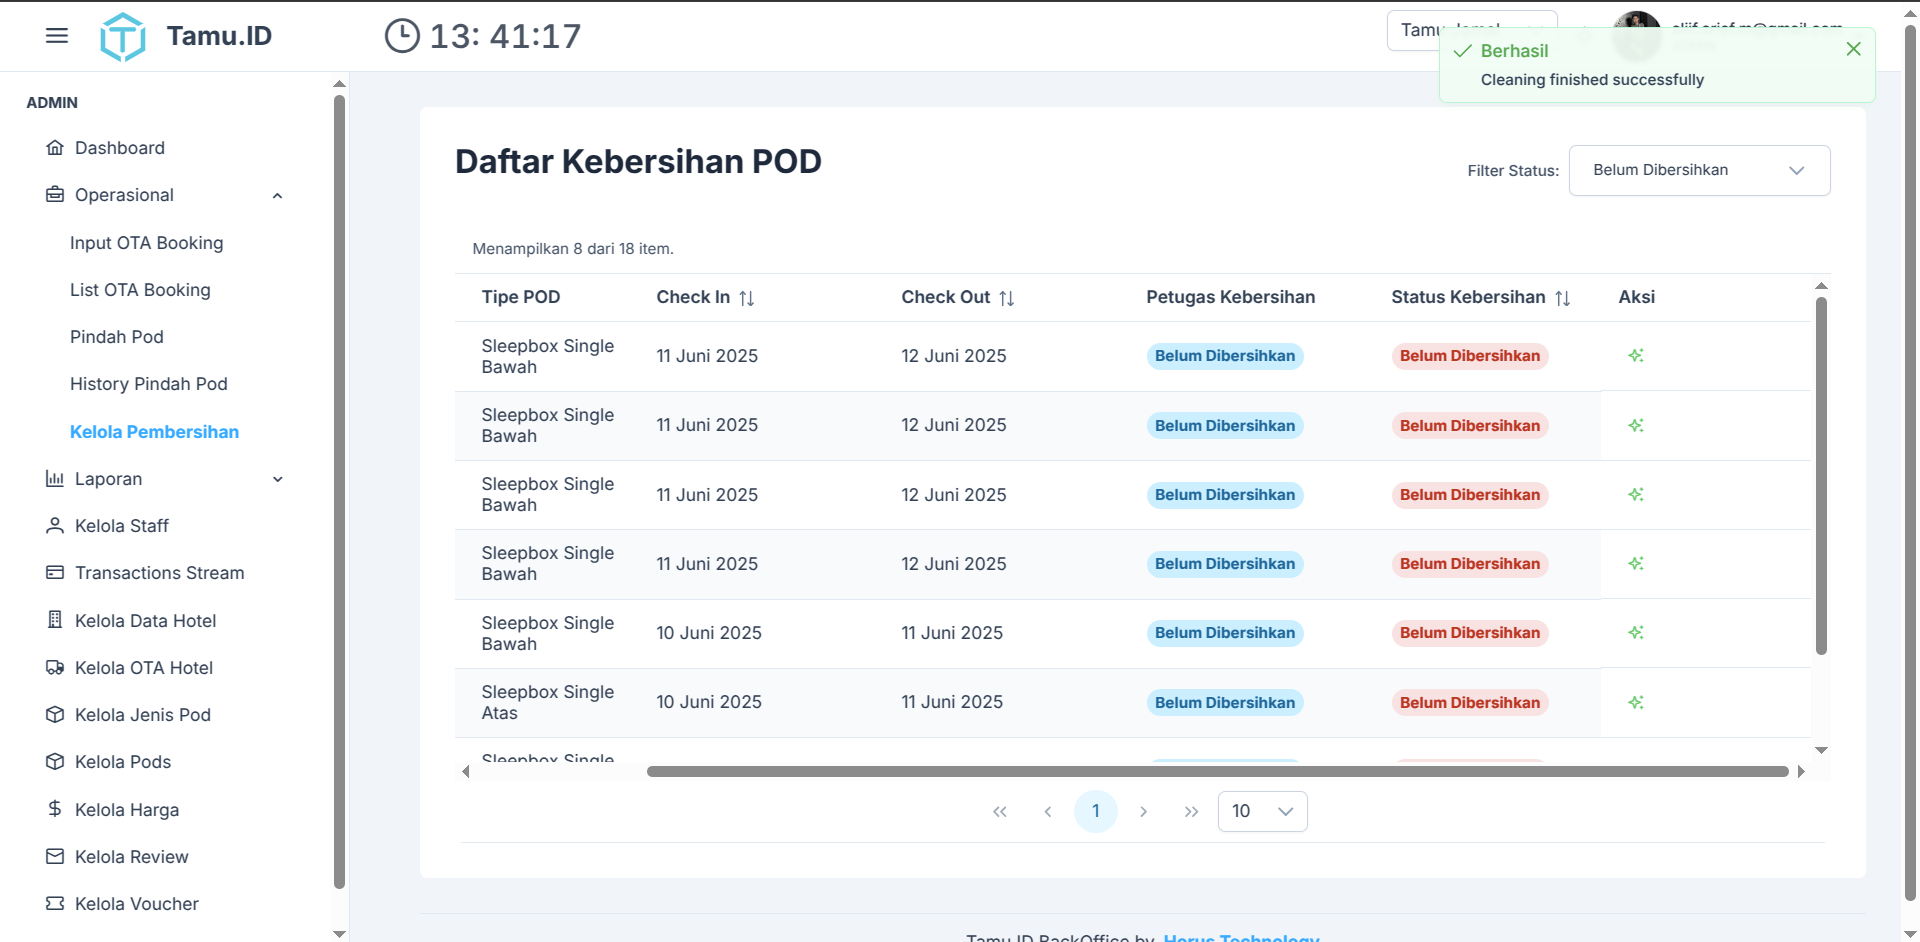
\includegraphics[width=\textwidth]{images/halaman-admin/list-harus-dibersihkan.png}
    \caption{Tampilan Halaman Daftar Pod yang Harus Dibersihkan}
    \label{fig:halaman-daftar-pod-harus-dibersihkan-admin}
\end{figure}

Setelah tamu check-out, admin dapat melihat daftar pod yang harus dibersihkan pada halaman daftar pod yang harus dibersihkan seperti pada gambar \ref{fig:halaman-daftar-pod-harus-dibersihkan-admin} dan melakukan tindakan seperti membersihkan pod tersebut.

\begin{figure}[H]
    \centering
    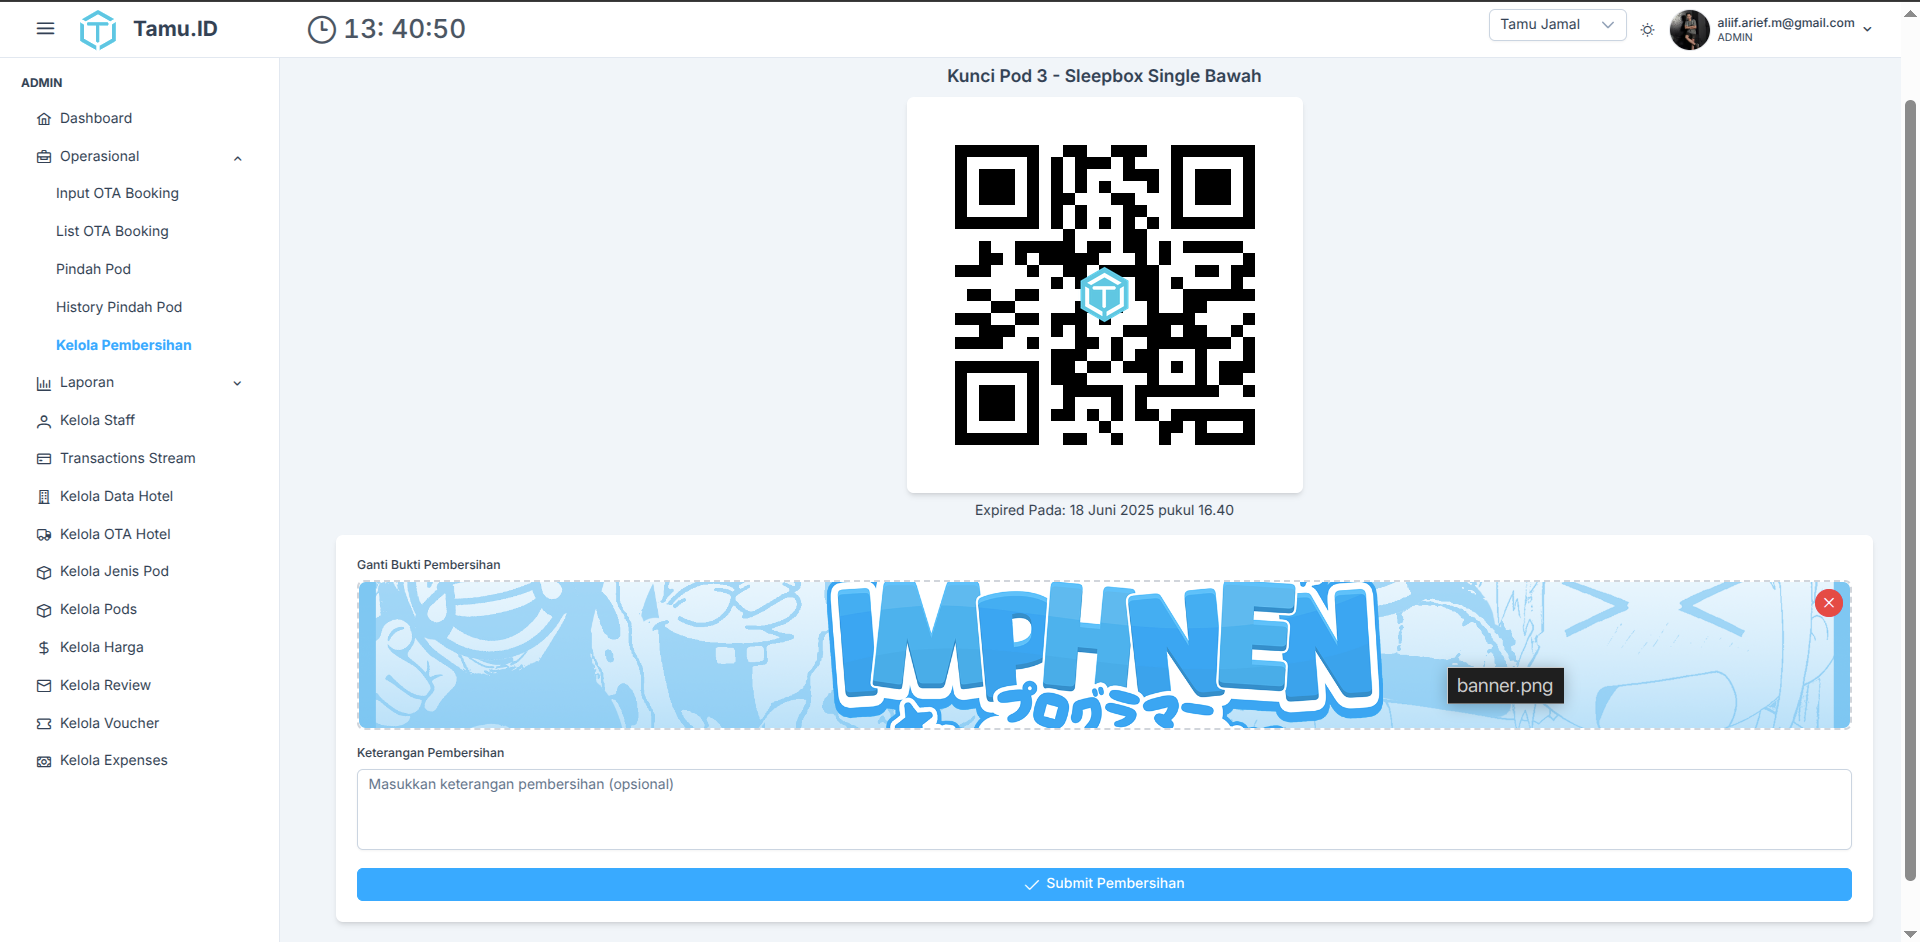
\includegraphics[width=\textwidth]{images/halaman-admin/proses-pembersihan.png}
    \caption{Tampilan Halaman Proses Pembersihan Pod oleh Admin Cabang}
    \label{fig:halaman-proses-pembersihan-admin}
\end{figure}

Pada gambar \ref{fig:halaman-proses-pembersihan-admin} adalah tampilan halaman proses pembersihan pod oleh admin cabang.

\begin{figure}[H]
    \centering
    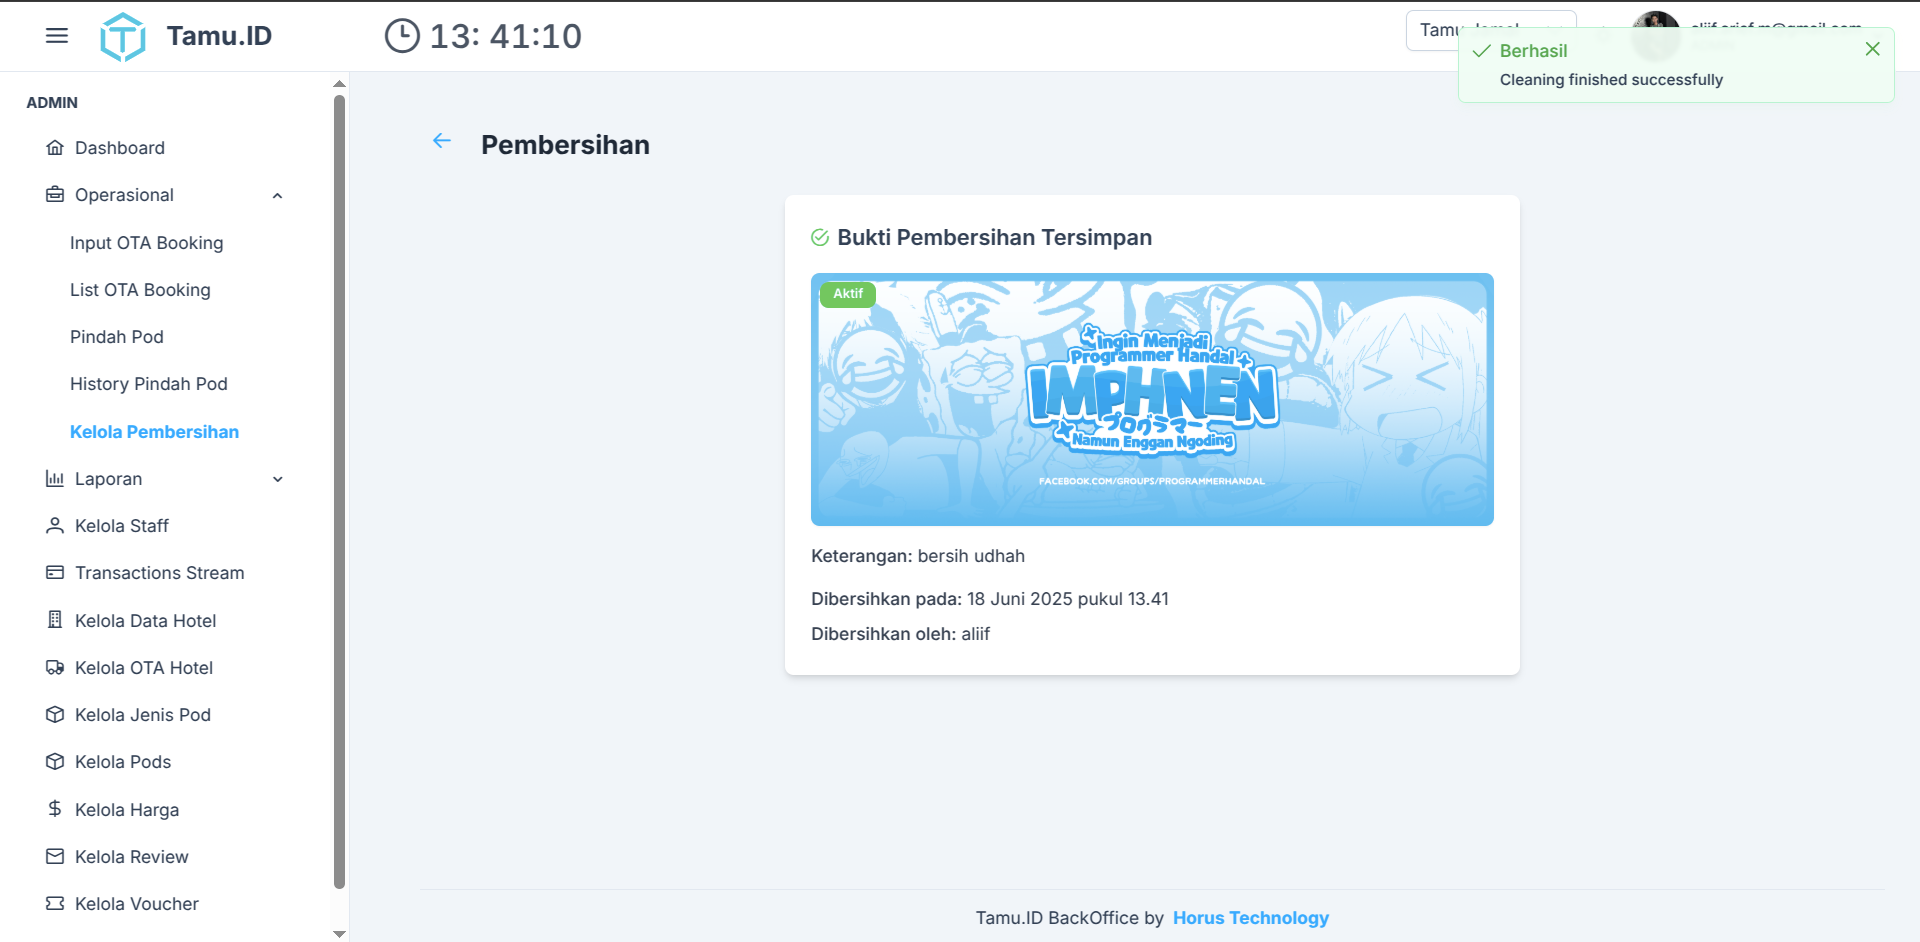
\includegraphics[width=\textwidth]{images/halaman-admin/selesai-pembersihan.png}
    \caption{Tampilan Halaman Pod Selesai Dibersihkan oleh Admin Cabang}
    \label{fig:halaman-pod-selesai-dibersihkan-admin}
\end{figure}

Setelah proses pembersihan selesai maka tampilan akan berubah menjadi seperti pada gambar \ref{fig:halaman-pod-selesai-dibersihkan-admin}.


\begin{figure}[H]
    \centering
    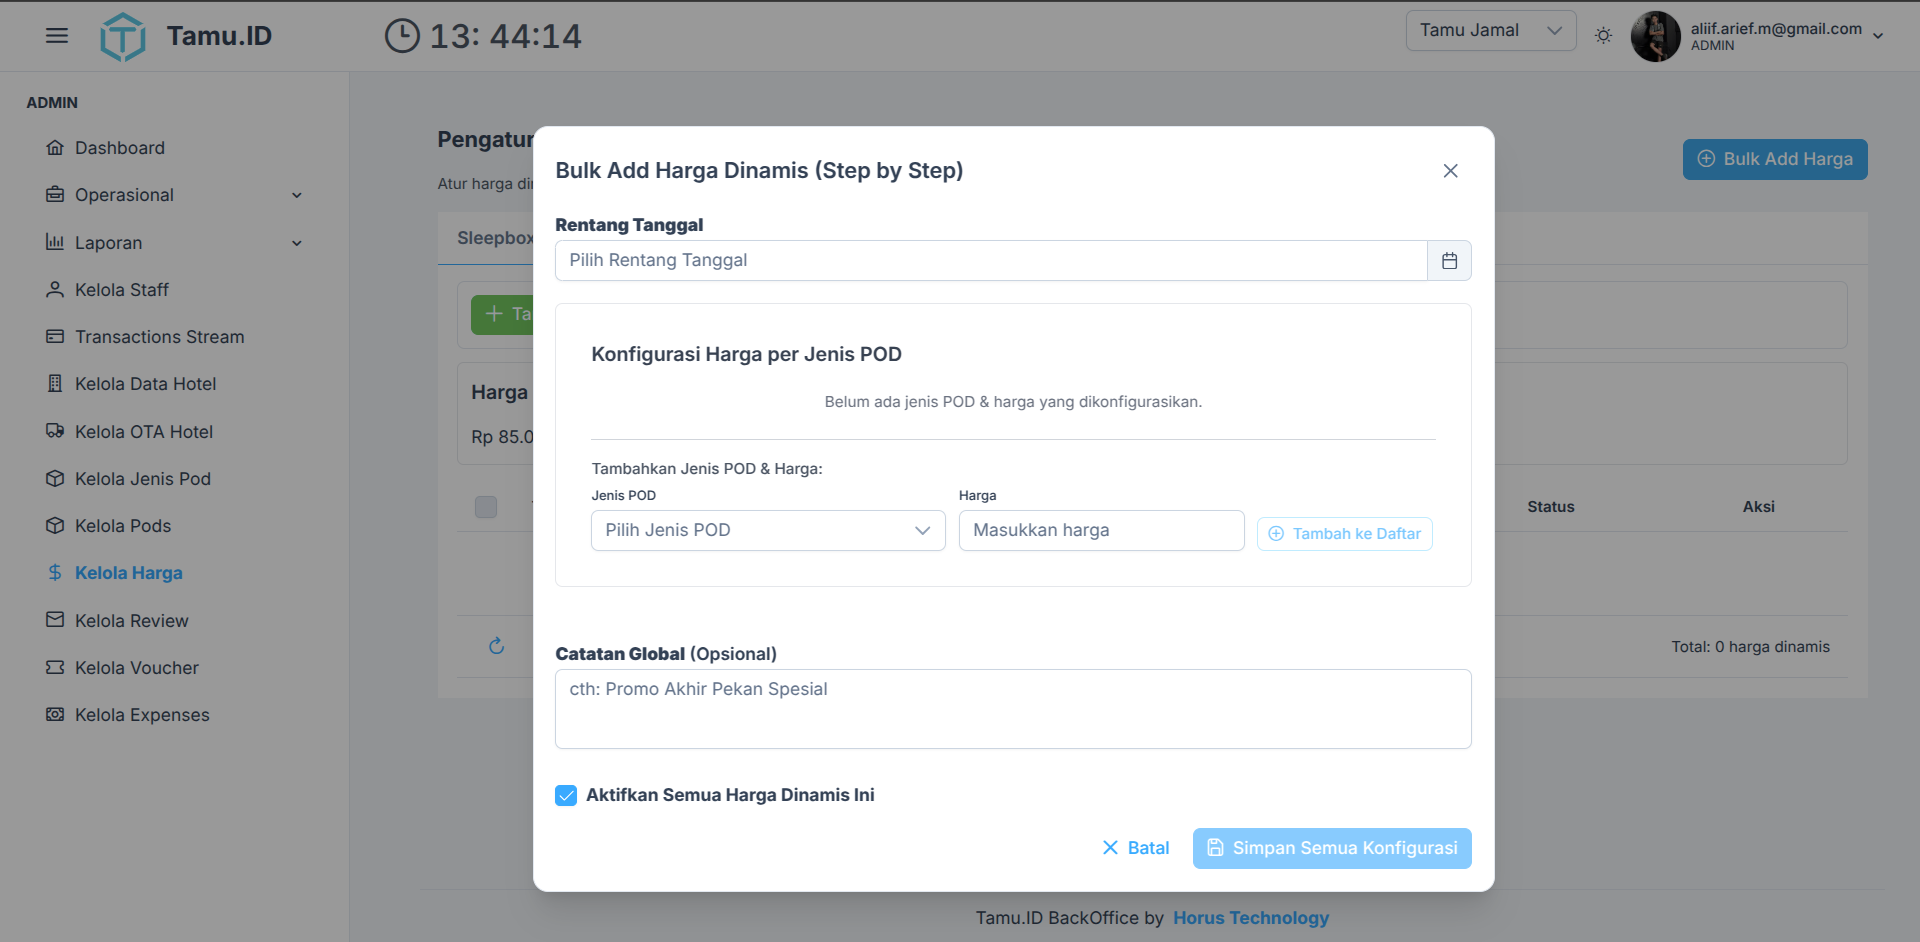
\includegraphics[width=\textwidth]{images/halaman-admin/hargadinamis.png}
    \caption{Tampilan Admin Kelola Harga Dinamis Cabang}
    \label{fig:halaman-admin-kelola-harga-dinamis}
\end{figure}

Pada gambar \ref{fig:halaman-admin-kelola-harga-dinamis} adalah tampilan halaman admin cabang untuk mengelola harga dinamis. Pada halaman ini, admin dapat mengatur harga dinamis untuk cabang yang dikelola. Harga dinamis ini akan digunakan untuk menentukan harga reservasi tergantung pada tanggal reservasi dan jenis pod yang dipilih oleh tamu. Hal ini dapat membantu admin dalam mengelola harga reservasi dan memastikan bahwa harga yang ditawarkan sesuai dengan kondisi pasar.

\begin{figure}[H]
    \centering
    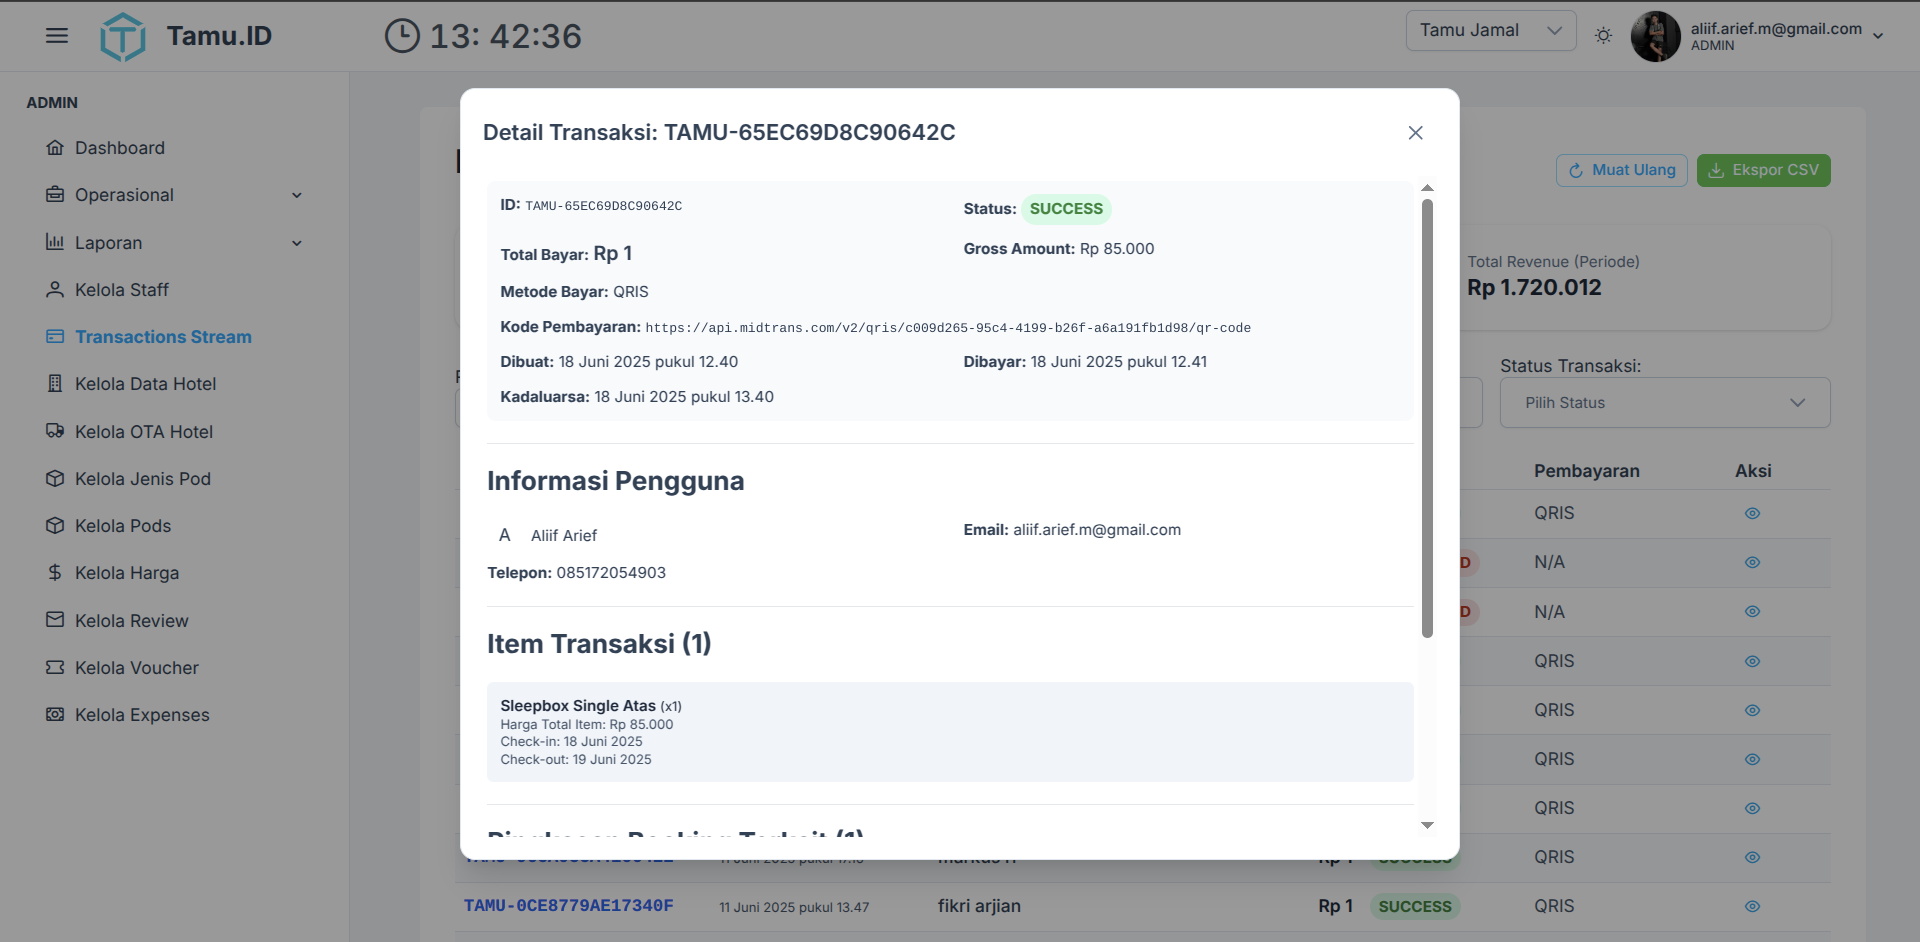
\includegraphics[width=\textwidth]{images/halaman-admin/transaksi.png}
    \caption{Tampilan Transaksi pada Cabang}
    \label{fig:halaman-transaksi-cabang}
\end{figure}

Pada gambar \ref{Tampilan Transaksi pada Cabang} adalah tampilan dimana Admin dapat melihat list dan detail transaksi yang terjadi untuk pod pada cabang yang ia kelola untuk visibilitas operasional yang lebih baik.

\begin{figure}[H]
    \centering
    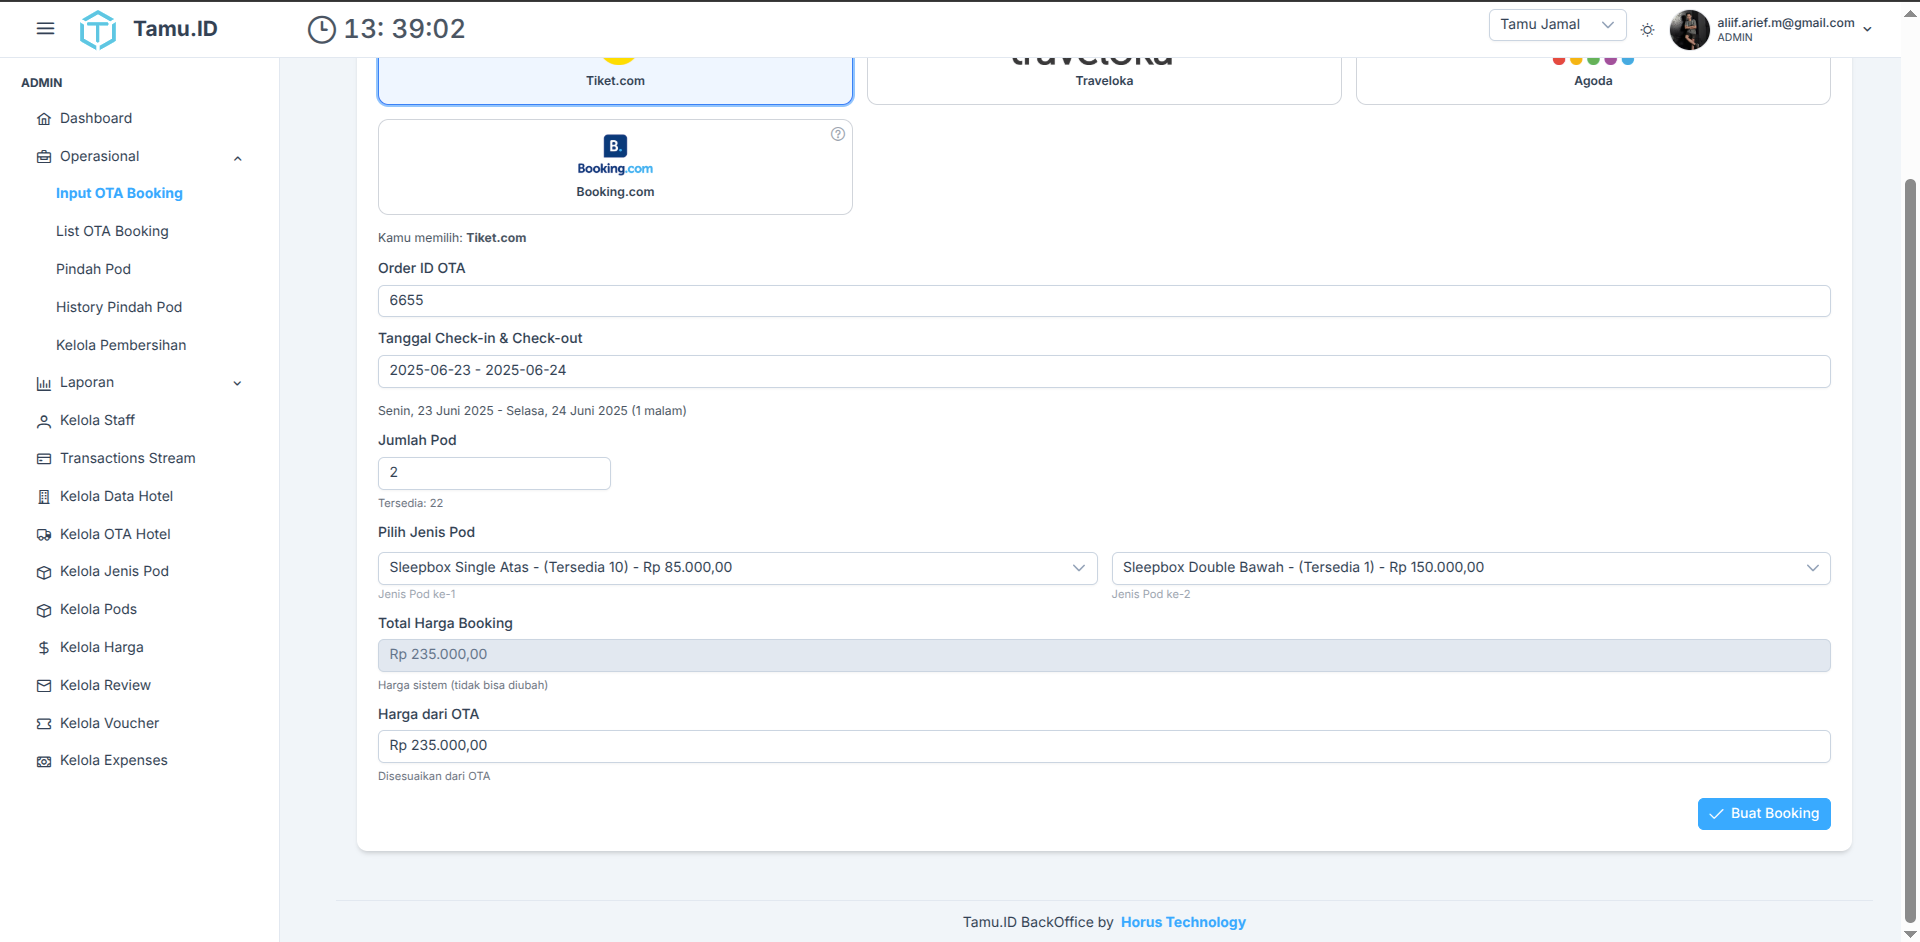
\includegraphics[width=\textwidth]{images/halaman-admin/input-ota.png}
    \caption{Tampilan Input \textit{OTA} pada Cabang}
    \label{fig:halaman-input-ota-admin}
\end{figure}


Integrasi antara \textit{Online Travel Agency} dan sistem Tamu.id belum berjalan secara otomatis sehingga ketika ada yang melakukan reservasi via \textit{Online Travel Agency} maka Admin harus menginputkan data reservasinya secara manual seperti pada gambar \ref{fig:halaman-input-ota-admin}.

\begin{figure}[H]
    \centering
    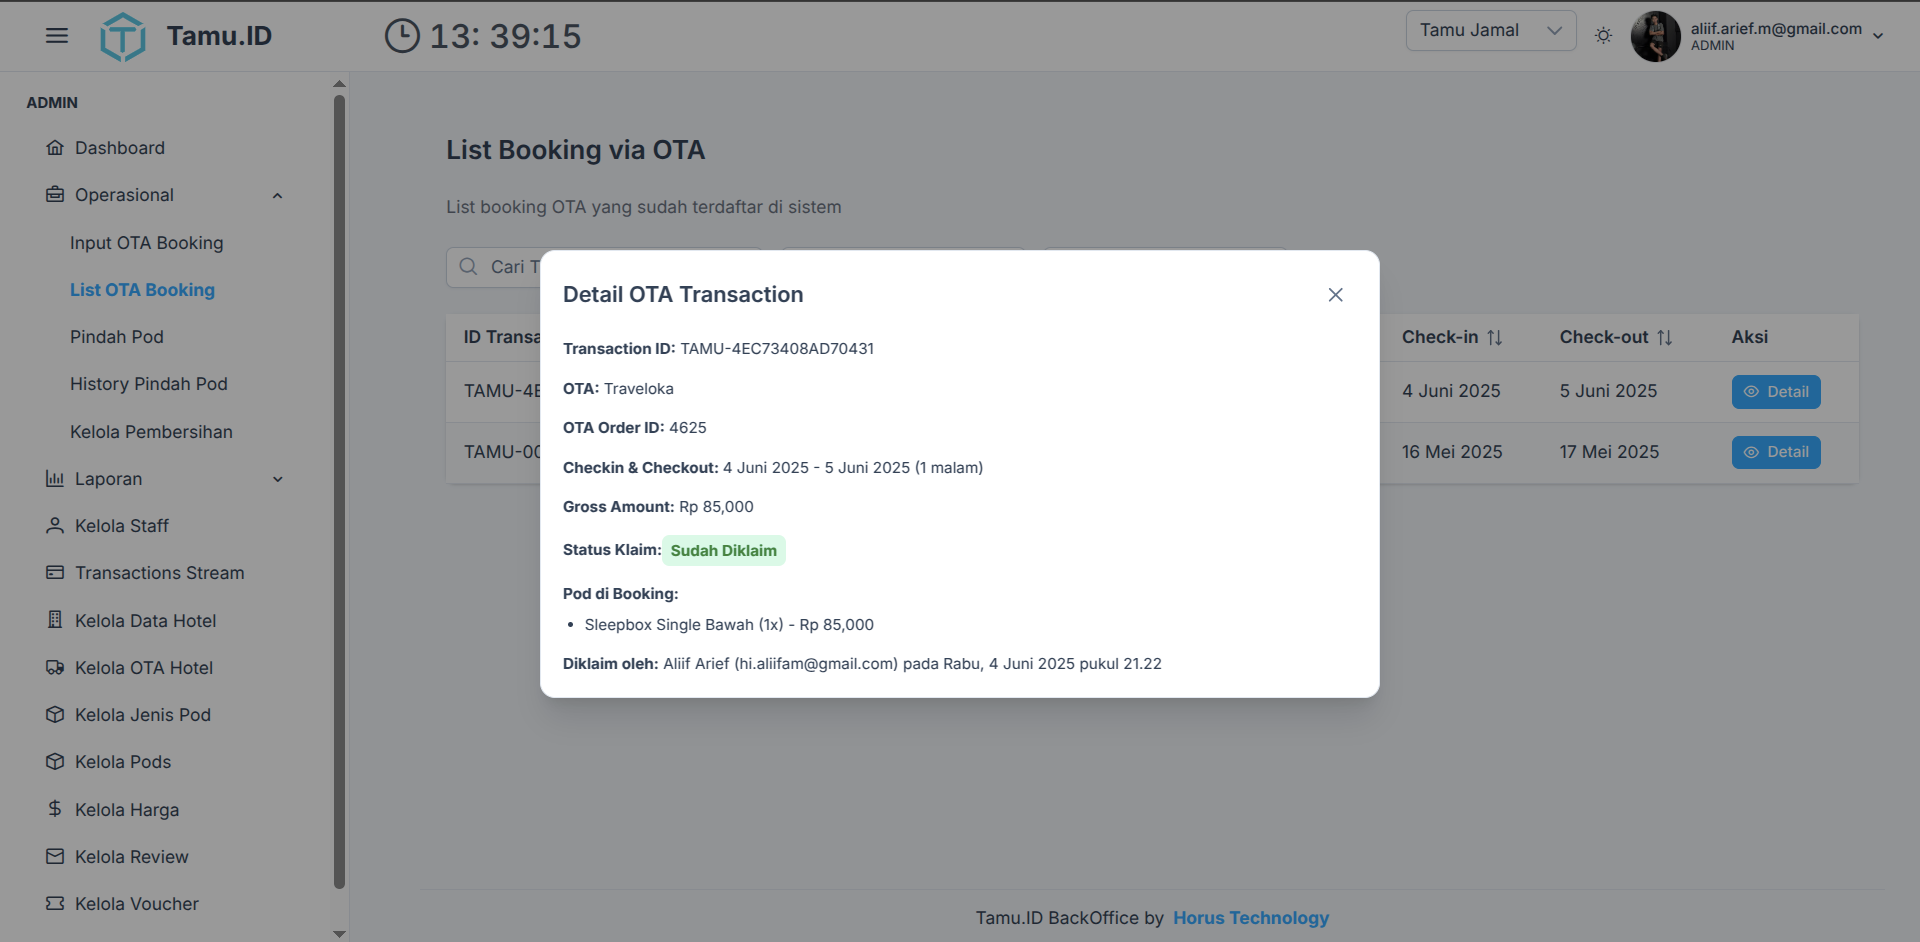
\includegraphics[width=\textwidth]{images/halaman-admin/lis-input-ota.png}
    \caption{Tampilan List Input \textit{OTA} pada Cabang}
    \label{fig:halaman-list-input-ota-admin}
\end{figure}


Pada gambar \ref{fig:halaman-list-input-ota-admin} merupakan halaman list data untuk reservasi \textit{User} yang dilakukan diluar platform yaitu dari \textit{Online Travel Agency}, untuk visibilitas dan kontrol yang lebih baik tentunya data - data yang sudah dimasukkan harus dapat terlihat dengan detail.
